\documentclass[11pt]{article}
%\documentclass[a4paper,11pt]{article}
\usepackage[a4paper, top=2cm, bottom=2cm, left=2cm, right=2cm]{geometry}
\usepackage[utf8]{inputenc}
\usepackage{eurosym}
\usepackage{amsmath}
\usepackage{amssymb}
\usepackage{amsthm}
\usepackage{enumitem}
\usepackage[normalem]{ulem}

%---------------------------------- refs ---------------------------
\usepackage[backend=bibtex,citestyle=alphabetic,bibstyle=alphabetic,
  giveninits=true,isbn=false,doi=false,url=false,
  maxbibnames=99]{biblatex}
%citestyle=numeric => numero
%citestyle=alphabetic => initiales des auteurs
%citestyle=authoryear => tous les auteurs + annee
\usepackage{multicol}
\usepackage{hyperref}
\hypersetup{
  colorlinks   = true, %Colours links instead of ugly boxes
  urlcolor     = blue, %Colour for external hyperlinks
  linkcolor    = blue, %Colour of internal links
  citecolor   = blue %Colour of citations
}
\usepackage[usenames, dvipsnames]{color}
\newcommand{\TM}[1]{\textcolor{black}{\underline{#1}}} %team member in references
%ugly hack to underline names while maintaining alphabetic order
\newcommand{\Rou}[1]{\textcolor{black}{\underline{#1}}} %team member in references
\newcommand{\Lab}[1]{\textcolor{black}{\underline{#1}}} %team member in references
\newcommand{\Coe}[1]{\textcolor{black}{\underline{#1}}} %team member in references
\newcommand{\Lac}[1]{\textcolor{black}{\underline{#1}}} %team member in references
\newcommand{\Ker}[1]{\textcolor{black}{\underline{#1}}} %team member in references
\renewcommand*{\bibfont}{\footnotesize}
\addbibresource{mybibliography.bib}

%---------------------------------- img ---------------------------
\usepackage{graphicx}
\usepackage{wrapfig}
\usepackage{subfig}
\graphicspath{{Images/}}
%
\usepackage[font={small},margin=1cm]{caption}
\usepackage{tikz}
\usetikzlibrary{spy}

%---------------------------------- misc ---------------------------
\usepackage{todonotes}
%---------------------------------- head ---------------------------
\usepackage{ifthen}
\usepackage{fancyhdr}
\pagestyle{fancy}
\setlength{\headwidth}{\textwidth}
\fancyhead{}
\lhead{\small PARADIS}
\chead{\small CES 23 (B.7, Axe 4)  - JCJC}
\rhead{\small AAPG ANR 2018}
%----------------------------------- macros ---------------------------
\newboolean{comments}
\setboolean{comments}{true} %"false" to disable comments
\newcommand{\Comments}[1]{\ifthenelse{\boolean{comments}}{{\scriptsize\em #1}}{}}
\newcommand{\DGtal}{\href{http://dgtal.org}{{\sc DGtal}}}
\newcommand{\DGtalTools}{\href{http://dgtal.org/tools/}{{\sc DGtalTools}}}
\newcommand{\IPOL}{\href{http://www.ipol.im/}{{\sc IPOL Journal}}}
\newcommand{\sage}{\href{http://www.sagemath.org/}{{\sc SageMath}}}

\newcommand{\dav}[1]{{\color{red} #1}}
\newcommand{\toUpdate}[1]{{\color{orange} #1}}

\newcommand{\ie}{{i.e.,~}}
\newcommand{\eg}{{e.g.~}}
\newcommand{\etal}{{et al.~}}

\newtheorem{Task}{Task}

%----------------------------------- math notation ----------------------
\newtheorem{Definition}{Definition}
\newtheorem{Conjecture}{Conjecture}
\newcommand{\Eq}[1]{Eq.~\ref{#1}}
\newcommand{\sect}[1]{sec.~\ref{#1}}

\newcommand{\Z}{{\ensuremath\mathbb{Z}}}
\newcommand{\R}{{\ensuremath\mathbb{R}}}
\newcommand{\Dig}{{\ensuremath\mathtt{D}_h}}
\newcommand{\Shapes}{\ensuremath{\mathbb{X}}}
\newcommand{\Shape}{\ensuremath{X}}
\newcommand{\BT}[1]{\ensuremath{\partial #1}}
\newcommand{\Set}{\ensuremath{\mathbf{S}}}
\newcommand{\Part}{\ensuremath{\mathbf{S}}}
\newcommand{\Plane}[2]{\ensuremath{\Pi_{#1,#2}}}
\newcommand{\UpperPlane}[2]{\ensuremath{\mathcal{P}^{+}_{#1,#2}}}
\let\vec\mathbf

%--------------------------------- WPs -----------------------------
\newcommand{\Risks}{\noindent
  \textbf{Risks, fall-back solutions: }}
\newcommand{\Success}{\noindent
  \textbf{Success indicators: }}
\newcommand{\Members}{\noindent
  \textbf{Members: }}

\newcommand{\WP}[5]{\noindent\fbox{
\begin{minipage}{0.98\linewidth}
\begin{tabular}{rp{1\textwidth}}
\textsc{\ref{wp#1}: }&    #2\\
\textsc{Main objective: }&    #3\\
\textsc{Members: }&    #4\\
\textsc{Deliverables: }&    #5\\
\end{tabular}
\end{minipage}}}

%% \newcommand{\WP}[2]{\noindent\fbox{
%% \begin{minipage}{0.98\linewidth}
%% \begin{tabular}{rp{1\textwidth}}
%% \textsc{Main objective: }&    1\\
%% \textsc{Members: }&    #2\\
%% \end{tabular}
%% \end{minipage}}}

%work-packages
\def \wpPPA {WP0}
\def \wpPattern {WP1}
\def \wpEstim {WP2}
\def \wpScale {WP3}
%\def \tExtend {T1} %obsolete
%\def \tSaddle {T2}

%----------------------------------- title ----------------------------
%\title{Title (French + English)}
%\author{}
%\date{}
%----------------------------------- doc ----------------------------
\begin{document}

%\maketitle
%\thispagestyle
\centerline{{\Large {\textbf{PAR}ameter-free \textbf{A}nalysis of \textbf{DI}gital \textbf{S}urfaces}}}
\centerline{\Large {(Analyse sans param\`{e}tre des surfaces digitales)}}
\bigskip
\centerline{PI: Tristan Roussillon}
\smallskip
\centerline{duration: 4 years}
\smallskip
\centerline{Requested funding: 260K\euro}
\smallskip

\Comments{Applicants are advised to use an easily readable document layout : A4 pages, Times 11 or equivalent, single spaced, 2cm margins, numbered pages.
  The project description must contain a maximum of 20 pages (including Gantt chart, overview of the requested funds and bibliography related to the project) and must be submitted in an unprotected PDF format.}

\Comments{Avant section 1:
 - summary table of persons involved in the project
 - Any changes that have been made in the full proposal compared to the pre-proposal : a priori pas de changement}


\abstract{
This project focuses on the geometry of digital surfaces, which are boundaries of voxel sets. These data mainly come from the segmentation of 3D digital images. Keeping the digital nature of the data is often an advantage. However, a drawback is its poor geometry at any resolution. The challenge is to enhance its geometry by estimating extra data for each surface element, such as a relevant normal vector.
The idea is to gather the geometrical information around each surface element within a patch of adaptive size: a piece of digital plane that locally fits to the digital surface. The covering of a digital surface by maximal pieces of digital plane is however hard because of their combinatorial explosion. An opportunity to make a breakthrough in this issue is the recent development of plane-probing algorithms. Based on these algorithms, we propose a new way of analyzing digital surfaces without any parameter. We expect a positive impact in graphics and 3D image analysis.
}

\tableofcontents

\begin{table}[h]
  \caption{Summary table of persons involved in the project}
\small
\centering
\begin{tabular}{|lcclc|}
\hline
LAST NAME \& first name & Position & Lab & Role in the project & Involvement (p.m) \\ \hline
\hline
COEURJOLLY David & DR & LIRIS & collaborator WP 2-3 & 5 \\ \hline
KERAUTRET Bertrand & MdC & LORIA & collaborator WP 3 & 12 \\ \hline
LABB\'E S\'ebastien & CR & LABRI & collaborator WP 0-1 & 12 \\ \hline
LACHAUD Jacques-Olivier & Pr & LAMA & collaborator WP 0,2-3 & 6 \\ \hline \hline
\textbf{ROUSSILLON Tristan} & MdC & LIRIS & \textbf{principal investigator} & \textbf{30} \\ \hline
\hline
\end{tabular}
\normalsize
\end{table}

\newpage

\section{Proposal's context, positioning and objectives}
\label{sec:context}

\subsection{Objectives and scientific hypotheses}
\label{sec:goals}

\Comments{Present the objectives and the research hypotheses ; present the scientific and technical barriers to be lifted ; present the expected results; if applicable describe any final products developed.}

\noindent\textbf{Context.}
In numerous fields of application, such as material sciences
or medical imaging, non-invasive acquisition devices such as magnetic
resonance, X-ray tomography or micro-tomography are required for
observation, measurements or diagnostic aids
(\eg \cite{Hildebrand1999,dcoeurjo_flin_ImPro}). %,dardenne2009variational}).
These acquisition devices usually generate volumic data, \ie
3D images, composed of regularly spaced data in a cuboidal domain.
3D volumes come from the segmentation of such 3D images.
They are also generated in scientific modelling because
numerous simulation schemes rely on the regularity of the data support
(\eg \cite{wojtan2007animating,jones2010directable,marechal2010heat}).

%% TRIS: je crois avoir garder l'esprit, mais j'ai reformule pour
%% pour éviter les répétition et mieux coller avec le reste

%% Thanks to non-invasive acquisition devices such as magnetic
%% resonance, X-ray tomography or micro-tomography, processing
%% subsets or partitions in 3D  binary volumes is crucial in
%% numerous fields of application, such as material sciences
%% or medical imaging (\eg \cite{Hildebrand1999,dcoeurjo_flin_ImPro,dardenne2009variational}).
%% Many volumetric acquisition devices generate regularly spaced
%% data and we have to process the geometry of regions defined as subsets in these
%%   3-D images.}  \dav{Alternatively, modeling mathematical objects or
%%   complex natural phenomena on voxel grids often lead to efficient
%%   solutions
%%   \cite{wojtan2007animating,jones2010directable,marechal2010heat}):
%%   one can exploit the regularity of the grid as a support for the
%%   numerical simulation schemes, or us the grid as an efficient
%%   datastructure to represent complex geometrical objects \cite{kampe2013sg,Villanueva:2016:SSS:2856400.2856420,JaspeVillanueva2017SSVDAG}.}

%% \dav{\sout{3D \dav{binary} volumes come from the segmentation of magnetic resonance, X-ray tomographic or micro-tomographic images. 
%% They are also generated in scientific modelling and by voxel
%% editors. }}


PARADIS is a project about the geometry of volume boundaries,
called \emph{digital surfaces} (fig.~\ref{fig:snow}). 
Keeping the digital nature of the data is an advantage
to do integer-only and exact computations,
to perform constructive solid geometry operations,
or to use efficient spatial data structures
(\eg \cite{kampe2013sg,Villanueva:2016:SSS:2856400.2856420,JaspeVillanueva2017SSVDAG}).
A drawback is its poor geometry, because at any resolution a digital surface is only 
made up of quadrangular surface element (\emph{surfel} for short) 
whose normal vector is parallel to one axis. 
Many tasks in computer graphics, vision and 3D image analysis require a richer geometry: 
rendering, surface deformation for simulation or tracking, precise geometric measurements, etc.
To perform relevant geometric tasks and 
to benefit from the above-mentioned advantages in the same time, 
we need to enhance the geometry of digital surfaces by estimating extra data for each surfel. 
This project focuses on estimations of local and first-order geometric quantities
such as normal vector direction.
%%, distance to boundary, coverage of the inner and outer incident voxels 
%%(see fig.~\ref{fig:2D} for a 2D illustration).  

\begin{figure}[hb]
  \centering
%
%\subfloat[]{ 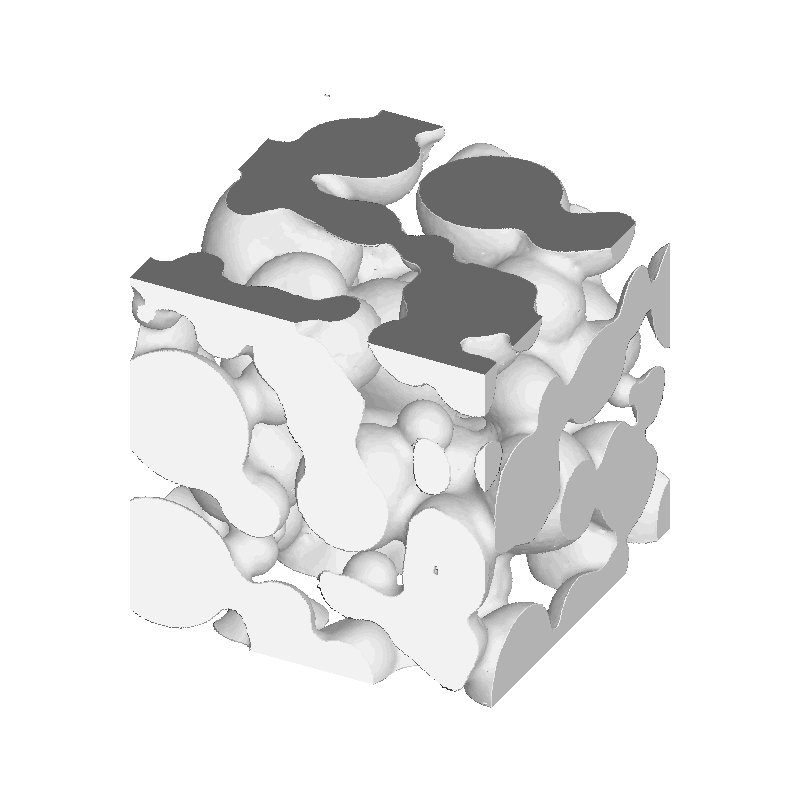
\includegraphics[height=0.2\textheight]{INH5_512_0}}
%
\subfloat[]{
\begin{tikzpicture}[spy using outlines={circle,yellow,magnification=2.5,size=2.8cm,connect spies}]
\node {\includegraphics[width=0.45\textwidth]{closeup-normals-3710x2112}};
\spy on (1.2,-0.2) in node [left] at (-0.95,-0.75);
\end{tikzpicture}
}
%
%
\subfloat[]{
\begin{tikzpicture}[spy using outlines={circle,yellow,magnification=2.5,size=2.8cm,connect spies}]
\node {\includegraphics[width=0.45\textwidth]{closeup-facets-3710x2112}};
\spy on (1.2,-0.2) in node [left] at (-0.95,-0.75);
\end{tikzpicture}
}
%
\caption{``ice-air'' interface in a micro-tomographic image of
  snow\protect\footnotemark. Local normal vectors are estimated
  at each corner (a) by computing relevant facets (b). This
  preliminary work does not extend the estimation to each surfel
  (see \sect{sec:estim:ds}). } 
\label{fig:snow} 
\end{figure}
\footnotetext{obtained by the 3SR Lab and CEN/CNRM - GAME URA 1357/M\'{e}t\'{e}o-France - CNRS, 
shared during ANR-11-BS02-009 DigitalSnow project.}

\noindent\textbf{Scientific bottleneck.}
The surface geometry within a patch around each surfel should be gathered to provide such estimations
-- \eg by polynomial fitting \cite{Cazals2005,Cazals2008}.
Almost all methods require at least one parameter that controls the size of the patch.  
On the other hand, this project aims at providing \emph{accurate} and \emph{parameter-free} estimators
based on a surface patch with \emph{adaptive} size.
%Note that accuracy will be evaluated in a \emph{multigrid-convervence} framework as described in section \ref{sec:wp}, WP2. 
Since we are looking for first-order estimations, the patch will be typically a piece of digital plane
that locally fits to the digital surface. %(fig.~\ref{sub:pattern}).
A challenge is to cover the whole digital surface by maximal pieces of digital plane. 
What makes the problem hard is that there is a combinatorial explosion
of maximal pieces of digital plane \cite{Sivignon2009} and that among them,
not all are tangent to the digital surface in a point set framework.  
An opportunity to make a breakthrough in this issue is the recent development
by the principal investigator and its collaborators of \emph{plane-probing}
algorithms \cite{LPRTCS2016, LPRDGCI2016, LPRJMIV2017}. These algorithms decide
on-the-fly how to probe the digital surface and make grow a piece of digital plane,
which is tangent by construction. The growth direction is given by both arithmetic and geometric properties.

\noindent\textbf{Objectives and expected results.}
PARADIS aims at analyzing digital surfaces. Three distinct goals can be highlighted:
\begin{enumerate}[label=(G\arabic*)]
  \item %[(G1)]
The first one is to study extra arithmetic and combinatorial properties
of plane-probing algorithms. We expect to design an ultimate plane-probing algorithm that
only probes a part of digital surface \emph{as small as possible} to provide a relevant facet.
A formal definition of what is meant by \emph{small} and a theoretical upper bound should be given.
In addition, we expect to correctly process non-convex parts by generating an underlying
minimal and connected piece of digital plane.  \label{goalppa} 
%(see WP0 and WP1 in section~\ref{sec:wp}, describing work packages).
 \item %[(G2)] 
The second goal is to derive \emph{efficient}, \emph{accurate} and \emph{parameter-free} estimators
of \emph{local} and \emph{first-order} geometric quantities: normal vector (and surfel area as a by-product),
distance to boundary, voxel coverage (fig.~\ref{fig:2D}). We expect to derive such estimators from
the above-mentionned plane-probing algorithm and provide a theoretical evaluation of their accuracy
with respect to resolution. \label{goalestim}  
%(WP2).
 \item %[(G3)] 
The third goal is to provide a method and a tool for an automatic and \emph{multiscale} analysis of digital surfaces,
based on the number or the size of the computed facets for several subsampled versions of the input 3D volume. 
We expect to develop a tool that provides, without any parameter, the scale at which noise is unlikely. Based on
this tool, we may add other features like a 3D normal estimator robust to noise.  \label{goalscale}
%(WP3). 
\end{enumerate}

\begin{figure}[hbt]
  \centering
\subfloat[]{ 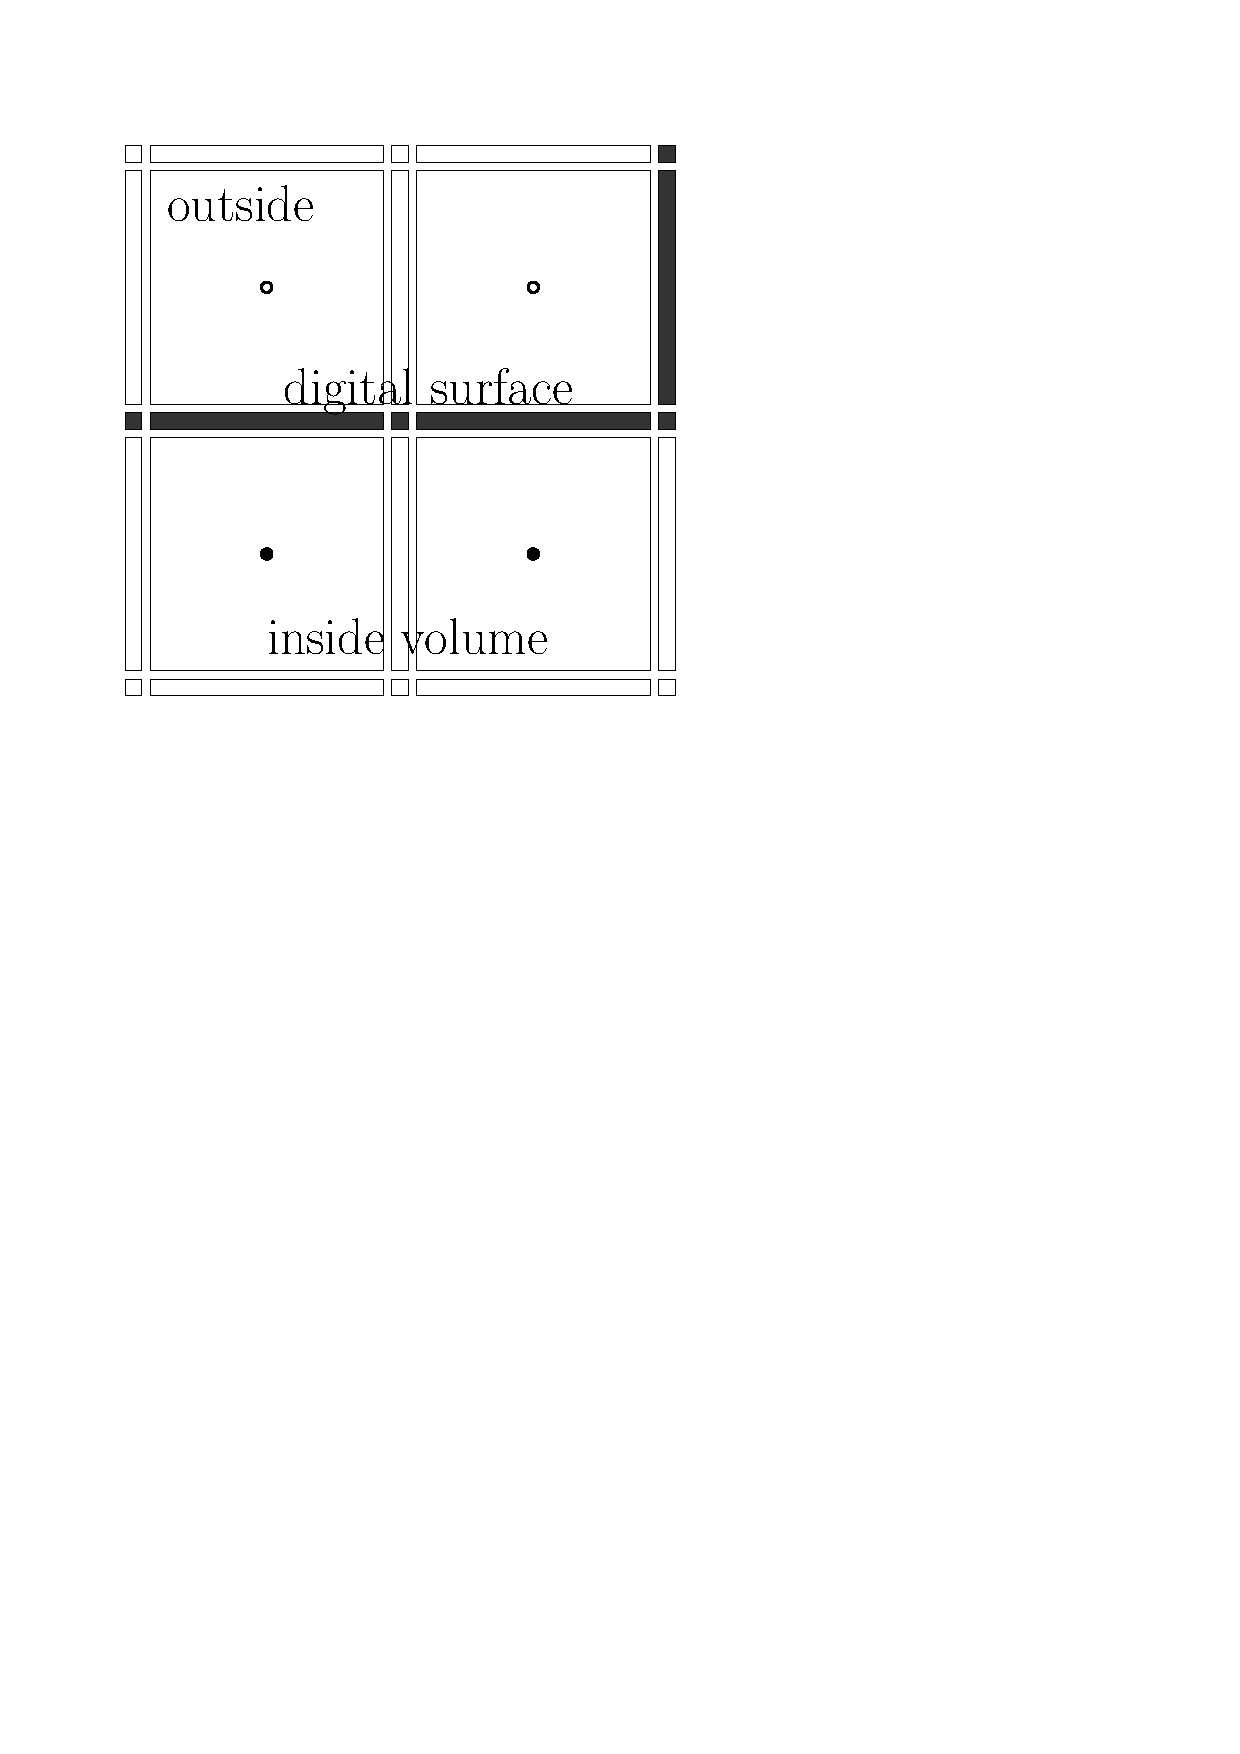
\includegraphics[width=0.13\textwidth,page=1]{square.pdf} } \hspace{0.05\textwidth}
\subfloat[]{ \includegraphics[width=0.13\textwidth,page=2]{square.pdf} } \hspace{0.05\textwidth}
\subfloat[]{ \includegraphics[width=0.13\textwidth,page=3]{square.pdf} } \hspace{0.05\textwidth}
\subfloat[]{ \includegraphics[width=0.13\textwidth,page=4]{square.pdf} } 
 \caption{2D illustration of a digital surface: voxels are big squares whose center is depicted by a black (resp. white) disk if it lies inside (resp. outside) the volume; surfels are elongated dark rectangles. We want to estimate a relevant normal vector at a given surfel (b), but also locally reconstruct a boundary perpendicular to this normal vector in order to derive distance and coverage estimations (c-d).} 
\label{fig:2D} 
\end{figure}

New algorithms, theoretical results and experimental studies will be gathered in papers submitted to
top venues or in peer-reviewed international journals. Plane-probing algorithms and derived estimators
will be implemented in the open-source C++ library {\DGtal}, whereas the tool will be added to {\DGtalTools},
a companion project of {\DGtal}, with an {\IPOL} paper for coding details.  

%sqdf \ref{goalppa} qsdf \ref{goalestim}, \ref{goalscale}. 
 
 %1-WP0: algorithm purely local, from any starting point, which leads to a reduced basis and retrieves any normal
%1-WP1: pattern generation: minimal number of tiles, connected, 
%2-WP2: estimateur + ordre de convergence theorique + applis ?
%3-WP3: outils qui prend un volume et sors un sous-échantillon non bruité, ou un ensemble de voxels à différentes tailles (publi IPOL)
%=> for each publication and implementation in DGtal. 

%transition not relevant here
%Since there are so many perspectives and paths to follow, this project needs to strengthen a team of experts by full-time workers in order to make the best of them. 

\subsection{Originality and relevance in relation to the state of the art}
\label{sec:art}

\Comments{Emphasise the ambitious nature of the proposal and the novelty of the research in relation to the state of the art ; show the possible contributions of project partners to the state of the art ; present any preliminary results. In the case of a project proposal following up on previous project(s) already funded by ANR or by another body, provide a summary of the results achieved and clearly describe the new issues raised and the new objectives set out in the light of the earlier project.}

In this section, we underline the novelty of the proposed approach in relation to the state of the art.  
We focus on the estimation of the normal direction, which is the most challenging task with the biggest impact. 
Other first-order quantities are either obtained as a by-product of the normal estimation (\eg surfel area)
or carry position information already approximated by the digital surface itself (\eg distance to boundary).
%In this last case, it seems unlikely that the accuracy could be improved by an order of magnitude. 

In addition, a digital surface is a quadrangular mesh. The vertex set consists of evenly spaced data points
whose coordinates are (half-)integer. This specific point cloud approximates a continuous 2-manifold under a
uniform noise model due to discretisation errors. That is why we review the most common methods for normal estimation
not only on digital surfaces, but also on meshes and point clouds.
%TODO nombreuses applications de normal estimation ce qui explique qu'il y ait beaucoup de travaux.  

%% Note that we do not present 2D estimators (\eg \cite{Provot2011,Esbelin2011,Esbelin2016}),
%% with the exception of \cite{Lachaud2007}, which is parameter-free and used in 3d estimators
%% \cite{Lenoir1996,Tellier1999,Lachaud2003}. 

\todo[inline]{Sébastien dit: L'utilisation de l'expression "state of the art"
est incorrecte dans le paragraphe suivant et pourrait laisser croire qu'on n'a
pas compris la question. Le
\url{https://en.wikipedia.org/wiki/State_of_the_art}, c'est ce qui se fait de
mieux dans la littérature par rapport à ce que nous on regarde. Ceci dit, la
première phrase plus haut ("In this section...") est correcte. Mais, ensuite,
on parle que ce ce que nous proposons, possiblement pas assez de ce qui se fait
deja dans le domaine pour resoudre ce genre de question et en quoi on est
different/mieux. Je crois que ce serait bien ici d'annoncer les sections 1.2.1,
1.2.2 et 1.2.3 et mentionner qu'elles répondent bien à ce qui est attendu: "In each of the three following sections, we describe the state of the art and explain the originality and relevance of our project."}

Since one goal of the project is to propose an accurate and parameter-free normal estimator,
we focus in this {\color{red} state of the art} on user-defined parameters and we check if
the estimator preserves sharp features and, for digital surfaces only, is
\emph{multigrid-convergent}, \ie the smaller the grid step,
the higher the resolution, the more accurate the estimator (fig.~\ref{fig:multi}). 

\begin{figure}[htbp]
  \centering
  \subfloat[$h=0.8$]{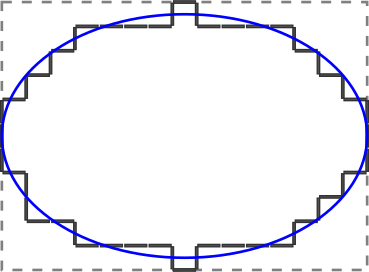
\includegraphics[width=0.25\textwidth]{conv08}}\hspace{0.05\textwidth}
  \subfloat[$h=0.5$]{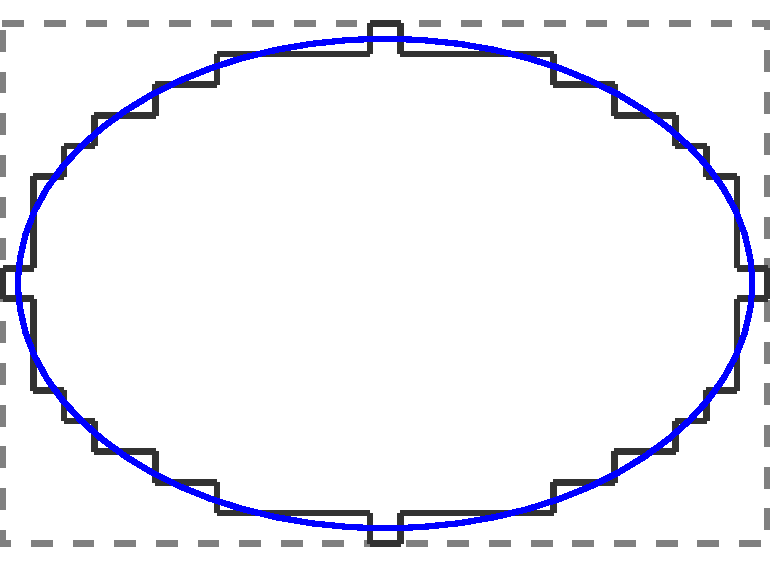
\includegraphics[width=0.25\textwidth]{conv05}}\hspace{0.05\textwidth}
  \subfloat[$h=0.2$]{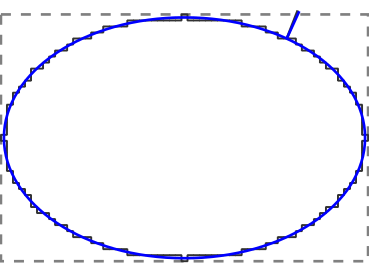
\includegraphics[width=0.25\textwidth]{conv02}}
  %% \subfloat[]{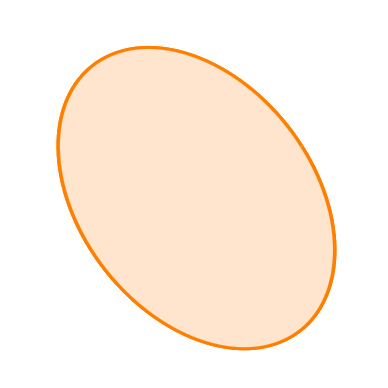
\includegraphics[width=3.5cm]{multi-ellipse-0}}
  %% \subfloat[]{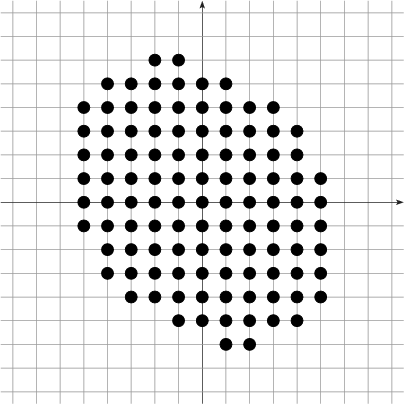
\includegraphics[width=3.5cm]{multi-ellipse-1}}
  %% \subfloat[]{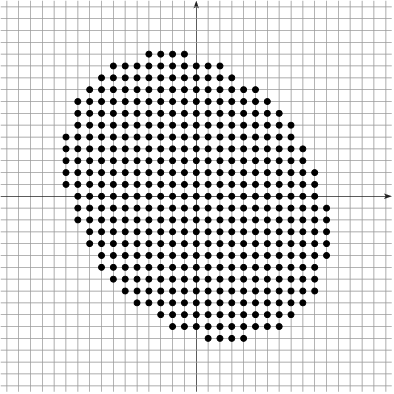
\includegraphics[width=3.5cm]{multi-ellipse-2}}
  %% \subfloat[]{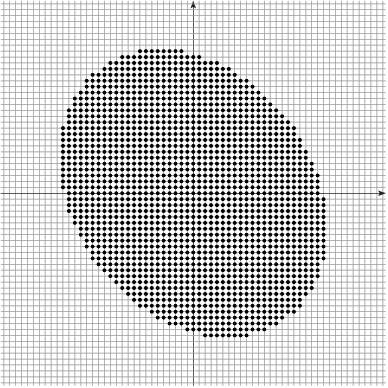
\includegraphics[width=3.5cm]{multi-ellipse-4}}
  \caption{Digitization of a 2D ellipse at a grid step $h$ taking decreasing values.
    A multigrid-convergent estimator is such that the estimated quantity at a point of a
    digital curve or surface gets closer to the one of the underlying continuous shape
    at a close enough point as $h$ tends to zero. Note that the length of the digital
    contour, which is equal to the perimeter of its bounding box (in dashed lines),
    is not multigrid-convergent, since it does not tend to the perimeter of the ellipse,
    but to the perimeter of its bounding box.}
  \label{fig:multi}
\end{figure}


%% \noindent\textbf{Digital surface and multigrid convergence.}

%% 3D volumes are collections of cubes. % of size $h$, called \emph{grid step}. 
%% Their topological boundary is a quadrangular mesh called \emph{digital surface}.
%% The vertex set consists of evenly spaced data points whose coordinates are
%% half-integer. This set approximates a continuous 2-manifold under a uniform
%% noise model. 
%% %TODO: Lachaud Thibert

%% Most of the time, when we are working with a digital surface, we are 
%% interested in the geometry of a continuous shape whose digitization
%% is the input 3D volume.
%% Formally, given a compact shape $X \subset \R^3$,
%% its digitization at grid step $h \in \R^+$ is $\Dig(X) := \{z \in \Z^3, hz \in X\}$.
%% If we denote the axis-aligned closed cube centered on $z \in h\Z^3$ and of size $h$ as $Q_z^h$,
%% the cube embedding of a digital set $Z$ at grid step $h$ is $\underset{z\in Z}{\cup}Q_z^h$.
%% Let $\partial_h X$ be the topological boundary of the embedding of the digitization of $X$: 
%% \[
%% \partial_h M := \partial \Big( \underset{z\in\Dig(X)}{\bigcup}Q_z^h \Big).
%% \]

%% We expect that a given geometric quantity, such as a normal vector,
%% computed at a point of a digital surface ($\partial_h X$),
%% is close to the one of the underlying continuous shape ($X$) at a close enough point. 

%% \begin{Definition}[multigrid-convergent estimator \cite{Coeurjolly2012}]
%%   \label{def:multigrid-convergence2}
%%   The estimator $\hat{Q}$ is {\em multigrid-convergent} for the family
%%   {\Shapes} if and only if, for any shape $X \in \Shapes$,
%%   there exists a grid step $h_X>0$ such that the estimate
%%     $\hat{Q}(\Dig(X),y,h)$ is defined for all
%%   $y \in \partial_h X$ with $0<h < h_X$, and for any $x \in \BT{X}$,
%%   \begin{equation*}
%%     \forall y \in \partial_h X \text{~with~} \| y - x \|_1 \le h, \quad
%%     \hat{Q}(\Dig(X),y,h) - Q(X,x) | \le \tau_{X,x}(h),
%%   \end{equation*}
%%   where $\tau_{X,x}: \R^{+*} \rightarrow \R^+$ has null limit at
%%   $0$.
%%   %% This function defines the speed of convergence of $\hat{Q}$
%%   %% toward $Q$ at point $x$ of $\BT{X}$. The convergence is {\em uniform} for
%%   %% $X$ when every $\tau_{X,x}$ is bounded from above by a function
%%   %% $\tau_X$ independent of $x \in \BT{X}$ with null limit at $0$.
%% \end{Definition}

%% The accuracy of a multigrid-convergent estimator depends on the grid step:
%% the smaller the grid step, the more accurate the estimator. 

\subsubsection{Normal estimation on point clouds, meshes and digital surfaces}
\label{sec:estim:all}

%interet des normales
Numerous tasks rely on the quality of the normal estimation in point clouds, such as
surface reconstruction, scene understanding or point-based rendering to name a few.
In surface fairing or mesh denoising, a common approach is to first compute a relevant
normal field and then evolve the mesh to match the smoothed normals.
Hence, a lot of normal estimation methods have been proposed. 

\noindent\textbf{Fitting.}
\citeauthor*{Hoppe1992} estimate the normal at a given data point by computing
the least squares best fitting plane to a point set within a neighborhood
around the point of interest \cite{Hoppe1992}.
Other fitting surfaces have been used too, such as jets, \ie truncated Taylor expansion
of a surface expression \cite{Cazals2005,Cazals2008}. 
All fitting methods first consist in collecting the points used for the fitting.
In the mesh case, a breadth-first search visits the neighbors until enough points
have been collected. In the point-cloud case, we typically resort to the k-nearest-neighbors
strategy. In both cases, the number of points to collect is usually a user-defined parameter.
Even if some heuristics are proposed to select it automatically \cite{Hoppe1992,Cazals2005},
these methods tend to smooth sharp features, and thus fail to correctly estimate normals
near edges.  

%\cite{Provot2011} ?

%In 3d, a straightforward application
%of \cite{Cazals2005}[Theorem 3] to digital surface shows that a polynomial fitting of degree $n$
%estimates the coefficients of the unit normal vector in $O(h^n)$.
%TRIS probablement faux

\todo[inline]{"first use", "propose", "propose", "has been proposed": Choisir si on parle de la littérature au passé ou au présent et être cohérent. (Perso, je prefere le passe).}

\noindent\textbf{Voronoi diagram.}
Instead of approximating the tangent space, another familly of methods focuses on the
Voronoi diagram to estimate at best the orthogonal space. \citeauthor*{Amenta1999} first use the
furthest vertex of the Voronoi cell to estimate the normals of point clouds \cite{Amenta1999}.
In order to get more stable estimates, \citeauthor*{Alliez2007} propose to apply linear fitting
to the Voronoi cell or to the union of Voronoi cells into a neighborhood \cite{Alliez2007}. 
\citeauthor*{Merigot2011} propose an improvement %, called Voronoi Covariance Measure (VCM),
by taking a weighted average of covariance matrices of Voronoi cells instead of
taking the covariance matrix of their union \cite{Merigot2011}. In their method,
only the intersection between the Voronoi diagram and a ball around the data point
are taken into account in order to get purely local information about the surface geometry.
A digital variant has been proposed by \citeauthor*{Cuel2015} \cite{Cuel2015}. 

\noindent\textbf{Integral invariants.}
In the mesh case, another method sums up the surface geometry within a ball by 
computing integrals over the intersection between the ball and the volume
bounded by the mesh \cite{Pottmann2009}. The covariance matrix of the intersection set 
provides a way to estimate principal curvatures, principal directions and normal direction.
A digital variant has been proposed by \citeauthor*{Lachaud2017} \cite{Lachaud2017}.
%
Note that the ball radius is a user-defined parameter in these
methods. In addition, the ball radius is usually the same for
the whole digital surface and completely ignore its features.
The above-mentionned digital variants \cite{Cuel2015,Lachaud2017}
are multigrid-convergent for digitization of smooth shapes if
the radius is conveniently chosen with respect to
the grid step.
%% TRIS: je trouve cet ajout poins pertinent (curvature estimator) et redondant avec la suite
%% \dav{In dimension 2, multigrid convergent
%%   parameter-free integral invariant curvature estimators can be
%%   derived \cite{Coeurjolly2014IIfree} but  extension to 3-D surfaces
%%   is not trivial (see below).}
%setting the ball radius from the
%  digital object boundary characteristics. Heuristics have been given
%  in 3-D but it is still an open problem whether multigrid convergent
%  and parameter-free curvature or normal vector estimators exist in 3-D.}

\noindent\textbf{Convolution.}
Starting from raw normal vector estimations (\eg unit
vectors perpendicular to surfels), several approaches refine the
estimation by convoluting the raw normals using a given smoothing
kernel. This technique has been proposed on digital curves
\cite{Esbelin2011,Esbelin2016} and surfaces
\cite{papierthese,Fourey2009} with the following drawbacks:
the user must specify the kernel parameters, including its size,
and the treatement, which is usually isotropic, smoothes out
sharp features. However, if the kernel size is some function of the
grid step, multigrid convergence can be obtained in 2D \cite{Esbelin2011}.
In mesh denoising, more advanced local filters, such as the bilateral one,
are used to preserve sharp edges and corners, but several parameters
are user-defined \cite{fleishman2003bilateral,zheng2011bilateral}.

\noindent\textbf{Variational approaches}. Another but similar approach
consists in minimizing a global energy function instead of applying a
local, iterative scheme. These techniques start from a raw estimation
of the normal vector field and use a complex variational scheme to obtain
a piecewise smooth regularization of the input field. The literature is
vast on this subject, see for instance \cite{zhang2015variational}. 
Applied to digital surfaces, robust and piecewise smooth normal vector fields
are obtained \cite{CoeurjollyFGL16}, but the multigrid convergence is not
discussed and the algorithm is time consuming. 

%% We conclude this
%%   overview by variational approaches aiming to denoise a surface or a
%%   normal vector field while preserving some features. Most techniques
%%   start from a raw (isotropic) estimation of the normal vector field
%%   and minimize an energy function to obtain a close piecewise smooth
%%   regularization of the input field. The literature is large on this
%%   subject, see \cite{CoeurjollyFGL16,zhang2015variational} for recent
%%   papers. These techniques can be seen as post-processes of a raw
%%   estimate and require complex schemes to solve the variational
%%   problem. Applied to digital surfaces, we obtain very robust and
%%   smooth normal vector field but the algorithm is time consuming and
%%   we are losing the pointwise multigrid convergence property.}

\noindent\textbf{Randomized Hough Transform.}
Finally, let us mention also probabilistic methods based on the Randomized Hough Transform.
Boulch and Marlet considered many random triples of data points in a neighborhood
and bin their normal direction into a spherical histogram \cite{Boulch2012}.
Maximal vote provides the normal estimate. However, their method has many input parameters,
the first of which is the size or radius of the neighborhood. 


\subsubsection{Parameter-free and adaptive normal estimators on digital surfaces}
\label{sec:estim:ds}

All reviewed methods have drawbacks. The few methods that perform an anisotropic
treatment to preserve features may be complex to implement, time-consuming, with
many user-defined parameters. The simplest methods have at least one parameter
that controls the size of the neighborhood for the whole data set and smooth out
sharp features.  

On the other hand, the specificity of digital surfaces makes the design of parameter-free
and adaptive estimators possible. The trick is to perform a uniform fitting of the data points by a plane.
In addition, instead of specifying the number of data points \emph{a priori}, they are added
step by step, while a maximal admissible error is not reached. This threshold is not a user-defined
parameter, but a known constant, because the data points follow a known uniform noise model
in case of digital surfaces. In 2D, methods based on digital straight segments (DSSs) follow
this approach.

The set of maximal DSSs, \ie inextensible straight parts, can be computed by one scan of the
digital curve \cite{Feschet1999,Feschet2005} and provides a multigrid-convergent
normal estimator \cite{Lachaud2007} (and normal integration over the digital curve yields
also a multigrid-convergent length estimator \cite{Coeurjolly2004}). In addition to
convergence, this normal estimator has several other sought-after properties:
it preserves sharp features (fig.~\ref{fig:corner}) and local convexity \cite{Roussillon2011},
without any input parameter. 
In addition, asymptotic properties of maximal DSSs can be used to estimate the local amount
of noise along the digital curve \cite{Kerautret2012}.  
\begin{figure}[htbp]
  \centering
  \subfloat[]{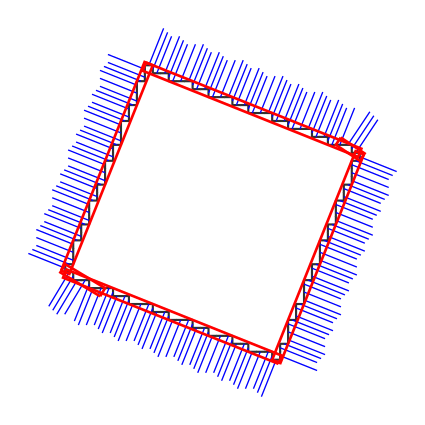
\includegraphics[width=0.3\textwidth]{square-g02-arith}}\hspace{0.05\textwidth}
  \subfloat[]{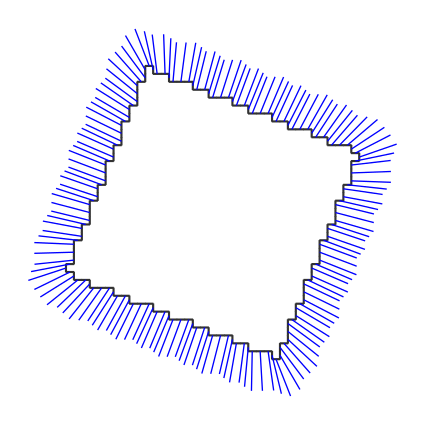
\includegraphics[width=0.3\textwidth]{square-g02-p50}}\hspace{0.05\textwidth}
  %\subfloat[]{\includegraphics[width=0.3\textwidth]{}} %TODO conv 3D
  \caption{Maximal DSSs provides a multigrid-convergent normal estimator that preserves sharp features (a). 
  Almost all other methods, such as convolution of the raw normals, smooth them out (b). }
  \label{fig:corner}
\end{figure}

In higher dimension, to the best of our knowledge, only one parameter-free normal estimator
has been proposed in 3D \cite{Lenoir1996,Tellier1999} and extended to nD \cite{Lachaud2003}.
It is based on maximal DSSs on 2D slices. Maximal DSSs provide windows of adaptive size
but the slicing truncates the geometric information and leads to
an artificial spatial variability because two neighbor surfels only
share one slice over two. 

Given an estimator with an input size parameter, a general strategy to automatically and adaptively select
the parameter value consists in taking the size of maximal DSSs. 
The idea of such hybrid method has been used first in \cite{Devieilleville2009}
for a comparative study of 2D normal estimators and then in \cite{Coeurjolly2014IIfree}
for mean curvature estimation by integral invariants.
In 2D, this strategy is quite interesting for higher-order estimators such as curvature,
but is totally disproportionate for normal estimation since maximal DSSs straightforwardly give a good estimator. 
In 3D, even if this hybrid method may be useful for normal estimation, its computation cost may be rather high,
because we must take into account the preprocessing cost to approximate the parameter value for each surfel,
and the cost of the original estimator without any optimization trick that takes profit of the neighboring
computations with the same parameter value, as done in \cite{Lachaud2017}. 

Finally, another possible approach is to mimic the 2D tool box by computing the set of
digital plane segments (DPSs) that locally fits to the digital surface. This approach
has been used for surface area estimation \cite{Klette2001}, reversible polyhedrisation
\cite{Sivignon2004} and normal estimation \cite{Charrier2011}. In the latter approach,
DPSs are initialized by a maximal circular neighborhood around a seed and then extended
without updating their normal vector. Even if it is a consistent definition of maximality,
this approach badly recover the geometry of the digital surface near sharp edges and corners. 
The challenge is to find how to scan the digital surface to efficiently recognize DPSs
whose size and shape adapt to the local geometry. 

\subsubsection{Digital plane segments: recognition and generation}
\label{sec:dps}

\noindent\textbf{Recognition of digital plane segments.}
A \emph{digital plane} is an infinite digital set that 
consists of several consecutive and parallel layers of coplanar points. 
It is defined by a (nonzero) normal $\vec{n} \in \Z^3$ and a position $\mu \in \Z$ as follows
\cite{reveilles1991}:  
\begin{equation}
  \label{eq:plane}
\Plane{\mu}{\vec{n}} := \{ \vec{x} \in \Z^3 \ | \ \mu \leq \vec{x} \cdot \vec{n} < \mu + \|\vec{n}\|_1 \}.
\end{equation}

Given a finite digital set $\Set$, the \emph{recognition problem} consists in providing
$\mu$ and $\vec{n}$ such that $\Set \subseteq \Plane{\mu}{\vec{n}}$ if they exist.
Note that such a recognition problem can have zero or infinitely many solutions.
One solution can be found in linear time, \ie in $O(|\Set|)$, by linear programming
and all solutions can be found in $O(|\Set|\log{(|\Set|)})$ by computational geometry tools.
See \cite{Brimkov2007} for a review on digital planarity.

However, we usually want to add data points step by step and incrementally update the solution
or the set of solutions. In this on-line framework, optimal algorithms are difficult
to implement and are in all probability slow in practice due to a high constant in the asymptotic
upper bound (see for instance \cite{Buzer2003}).
On the other hand, there exists fast geometrical algorithms but with higher theoretical bounds,
\eg \cite{Gerard2005, Charrier2008, Veelaert2012}.
%\cite{Gerard2009} preimage
%\cite{Stojmenovic1991} separation
%Provot2006, largeur

Actually, the main challenge is not so much to recognize DPSs, but more to find which data points
should be taken into account during the recognition process to obtain DPSs tangent to the digital
surface. In addition, as noted \cite{Charrier2011}, most inextensible digital planar sets are not
characteristics of the local geometry of the shape and finding the smallest subset which covers
the digital surface has been shown to be NP-complete \cite{Sivignon2009}.
Segmentation methods usually make a point set grow from a seed by a breadth-first search according
to some heuristics and decide whether the current set is a piece of digital plane or not
(see for instance \cite{Klette2001} or \cite{Sivignon2004}). 
%\cite{Provot2009} un peu different car parametre de bruit
The results are however highly dependent on the chosen heuristics.   

Until recently, artihmetic properties of digital planes did not help so much.
Pionneering incremental recognition algorithms based on arithmetic properties
\cite{Debled1994,Mesmoudi2002} are neither as easy-to-implement nor as fast as
purely geometric ones, such as \cite{Gerard2005}.  
The work of V. Berth\'{e} and T. Fernique \cite{Fernique2009,Berthe2011}, 
based on multidimensional continued fractions and desubstitution on words,
is quite interesting from a theoretical point of view. However, their algorithm,
which reduces a piece of digital surface until no transformation is possible,
is not of practical interest because it requires the whole point set to be known
in advance and must be coupled with another recognition algorithm to conclude
at the last step.  

\noindent\textbf{Preliminary results: plane-probing algorithms.}
A novel approach has been proposed by the principal investigator and its collaborators
\cite{LPRTCS2016, LPRDGCI2016, LPRJMIV2017}. 
Given a digital plane $\Plane{\mu}{\vec{n}} \subset \Z^3$
and a starting point $\vec{p} \in \Set$, 
a \emph{plane-probing algorithm} computes the parameters of a digital plane $\Plane{\mu'}{\vec{n}'}$
containing $\vec{p}$ by sparsely probing $\Plane{\mu}{\vec{n}}$ with the predicate
``is $\vec{x}$ in $\Plane{\mu}{\vec{n}}$?''. The parameters of $\Plane{\mu}{\vec{n}}$
and $\Plane{\mu'}{\vec{n}'}$ are expected to be equal when the algorithm terminates.
%for any $\vec{p} \in \Plane{\mu}{\vec{n}}$. 

What makes plane-probing algorithms promising is that they decide on-the-fly how
to probe the digital surface and make grow a piece of digital plane, which is
tangent by construction. 
The first algorithm of this kind has been proposed in \cite{LPRTCS2016}.
Its principle is to deform an initial unit tetrahedron based at the starting point
with only unimodular transformations. Each transformation is decided by looking
mostly at a few points around the tetrahedron. These points are chosen so that
the transformed tetrahedron lies in $\Plane{\mu}{\vec{n}}$, with the same volume,
but closer to the upper plane
$\UpperPlane{\mu}{\vec{n}} := \{ x \in \R^3 \ | \ x \cdot \vec{n} = \mu + \|\vec{n}\|_1 \}$.
At the end of this iterative process, one face of the tetrahedron has an extremal
position in the plane and is thus parallel to $\UpperPlane{\mu}{\vec{n}}$.

New plane-probing algorithms have been proposed in \cite{LPRDGCI2016, LPRJMIV2017}. 
They also iteratively deform an initial tetrahedron and stop when one face is
parallel to $\UpperPlane{\mu}{\vec{n}}$ (see fig.~\ref{fig:ppa} for an illustration). 
%
\begin{figure}[htbp]
  \centering
  \subfloat[]{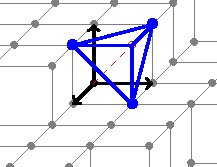
\includegraphics[width=0.17\textwidth]{triangle-1-2-5-0-0}}
  \subfloat[]{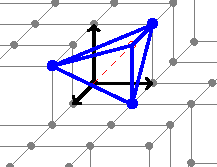
\includegraphics[width=0.17\textwidth]{triangle-1-2-5-0-2}}
  \subfloat[]{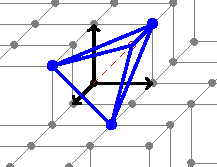
\includegraphics[width=0.17\textwidth]{triangle-1-2-5-0-4}}
  \subfloat[]{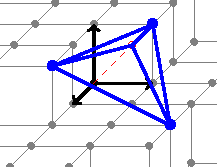
\includegraphics[width=0.17\textwidth]{triangle-1-2-5-0-6}}
  \subfloat[]{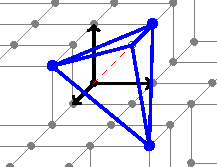
\includegraphics[width=0.17\textwidth]{triangle-1-2-5-0-8}}
  \caption{The current tetrahedron is depicted in blue. It is initialized at a corner (a) 
    and it is then deformed step by step by the \emph{R-algorithm} proposed in \cite{LPRJMIV2017} (b-e).
    When the algorithm terminates (e), the normal of the facet not incident to the fixed vertex
    is equal to the normal of the underlying digital plane, \ie $(1,2,5)$.}
    \label{fig:ppa}
\end{figure}
%
However, these new algorithms differ from the first work on several aspects.
First, they are simpler, because they repeat one simple operation instead
of several possible transformations depending on the current onfiguration
as in \cite{LPRTCS2016}.  
Second, one vertex of the evolving tetrahedron is a fixed point lying above the 
starting point and the opposite triangular facet (fig.~\ref{fig:ppa}). The position
of the evolving tetrahedron is thus better controlled than in \cite{LPRTCS2016}. 
Last, a geometric criterion is used so that the evolving tetrahedron is not
too much elongated during the computation.  

%surface
In addition, \cite{LPRJMIV2017} show how to use these algorithms
for digital surface analysis. One drawback of this preliminary work
is the processing of non-convex parts. This case requires to associate
a piece of digital plane to the tetrahedron.

%% by discretizing its triangular facet
%% not incident to the fixed point. Generating a relevant piece of digital plane
%% in the course of the computation may be a neater and more efficient
%% solution.  

%% Although it is a preliminary work with
%% several drawbacks that we expect to overcome in this project, some fall-back
%% solutions are detailed. 

%% For instance, a procedure for detecting planarity defects
%% is detailed.  and in case of non-convex configuration and propose several strategy 
%% We show how to detect convex/concave/inflexion zones onto a digital surfacewe show  , we also For some well-identified starting points, this algo- rithm stops and outputs only an approximation of the normal to P. We show how to detect such bad starting points and how to connect them to their corresponding facet

%reduction
%% For one variant, called $R$-algorithm, we experimentally observe
%% that the returned basis is reduced at least after every two steps and it is always reduced
%% when the algorithm terminates. This conjecture is not proved yet and it is one of our
%% future work to prove it.

\noindent\textbf{Discretization and generation.}
%generation de plans
%% Due to the analytical definition of digital plane (see \Eq{eq:plane}), it is
%% trivial to generate an arbitrary piece of digital plane. Indeed, it is enough to scan all
%% the digital point of a given domain and for each of them to check whether
%% it belongs to the digital plane or not. However the topological and
%% arithmetical properties of standard digital planes defined in \Eq{eq:plane}
%% make generation algorithms more efficient, using breadth-first
%% traversal and incremental computations.
Due to the analytical definition of digital plane, its topological and
arithmetical properties, we can efficiently generate an arbitrary piece
of digital plane using breadth-first traversal and incremental computations.
However, if the piece of digital plane is required to be projected into a
given polygon or simply a triangle as in \cite{LPRJMIV2017}, this approach
is not always possible, because acute angles can make the digital set disconnected. 

%discretisation de polygone en 3D
The standard analytical model provides a consistent way to discretize a $m$-simplex
in $n$D with topological guarentees, \ie into a $(n-1)$-connected, tunnel-free
and bubble-free point set \cite{Andres2003}. This model has been successfully
used for reversible polyhedrisation by \citeauthor*{Sivignon2004} \cite{Sivignon2004},
because they precisely find a way of building a polyhedron that can be
discretized into the input 3D volume according to this model.
%The resulting polyhedron has some very small facets and its vertices have rational coordinates.
In the framework of \cite{LPRJMIV2017}, this model, which generates a point set
centered around the $m$-simplex, requires to shift the triangular facet by half of the
digital plane thickness.

However, plane-probing algorithms allow to use totally different generation algorithms
based on multidimensional continued fractions (MCF), \eg \cite{Fernique2009,Jamet2016}. 
They indeed generate a sequence of unimodular matrices, each one mapping a tetrahedron to
the next one, just as MCF algorithms generate a sequence of matrices, each one mapping
a vector to the next one. As a result, we can either adopt a translation-union approach \cite{Jamet2016}
or use (dual) substitutions \cite{Fernique2009} in order to generate a piece
of digital plane whose geometry follows the matrix sequence. The topological and geometrical
properties of such a piece of digital plane is currently unknown and needs to be investigated. 

%TODO: image d'illustration avec matrix sequence ?


\subsection{Methodology and risk management}
\label{sec:methodo}

\Comments{Describe the methods and technical decisions, risks and fall-back solutions envisaged.}

Based on the previous discussion, we give a brief description of the project methodology.
The main risks are highlighted with their fall-back solutions (more details in the next section).  

\noindent\textbf{Methodology overview.}
%plane-probing algorithms sont une bonne approche pour etre tangent, local, sans parametre,
PARADIS aims at proposing a theoretical and practical framework for the automatic
analysis of digital surfaces. We believe that plane-probing algorithms give the right
direction to follow, because they provide a way to obtain a relevant piece of digital
plane that locally fits to the digital surface without any parameter. The normal direction
to this digital plane segment is expected to preserve sharp features and to be multigrid-convergent.
%and accurate even at low resolution.

The preliminary works \cite{LPRTCS2016, LPRDGCI2016, LPRJMIV2017}
currently suffer some limitations, but we already know several ways of
solving these problems. More details will be given in \sect{sec:wp}. 
%substitution bonne approche pour generer un motif au cours de l'algorithme
One issue arises when processing non-planar parts, especially non-convex ones.
In such cases, a sparse probing is not enough to correctly identify the underlying geometry
as reported in \cite{LPRJMIV2017}.
We believe that generating a piece of digital plane in the course of the computation will
not only solve this problem but also give new insights on the combinatorial structure
of DPSs. 
%This knowledge will be useful for both algorithm optimization
%and asymptotic analysis of linear parts.   

%lien avec env. conv. bonne approche pour preuve estimateur et analyse multi-echelle
An important achievement will be to derive a multigrid-convergent normal estimator.
Another one will be to develop an automatic tool that selects a locally noise-free scale.
Both achievements will be based on an asymptotic analysis of linear parts. Such analysis
will require a good understanding of the combinatorial structure of DPSs
but also a good understanding of the link between facets computed by plane-probing algorithms and
facets of (relative) convex hull. This approach has been adopted with success for digital
curves \cite{Lachaud2012} and we believe that it can be similarly applied to digital
surfaces with the help of plane-probing algorithms.
 
\noindent\textbf{Risk management.}
Preliminary works have considerably reduced the risks but have not eliminated them.
Main risks are classified below by goal: risks \ref{riskppa}, \ref{riskestim} and \ref{riskscale}
respectively correspond to goals \ref{goalppa}, \ref{goalestim} and \ref{goalscale}. 
\begin{enumerate}[label=(R\arabic*)]
  \item %[(G1)]
%algos pas parfaits: il en existe actuellement un 
%motif genere pas bons:
 %- on les genere apres coup en faisant une sorte de croissance de regions
 %- on traite les concavites avec un critere de separation
First, we may struggle to find the ultimate plane-probing algorithm or fail to do so.
If it happens, we will resort to the \emph{R-algorithm} \cite{LPRJMIV2017}, which
has interesting properties related to the locality of the probing, or a combination
of different but complementary plane-probing algorithms to make the best of them
as suggested in \cite{LPRJMIV2017}. We will lack provable properties but we will be able to still
develop practical algorithms in order to derive a parameter-free normal estimator.
%general approach
For instance, we can adopt the approach of \citeauthor*{Charrier2011} \cite{Charrier2011}
where we replace the initial isotropic neighborhoods by the digitization of the facets
returned by the R-Algorithm. Extending all these pieces of digital plane, we will obtain a
tangential cover that may be less sensitive to the initial step and from which we can
deduce an estimation of the normal vector field that better captures the geometry of
the digital surface near sharp edges and corners than the original method. \label{riskppa} 
\item %[(G2)]
%l'estimateur n'est pas convergent: peu probable, mais si ça arrive c'est que les motifs sont trop petits, il ne grandisse pas assez vite par rapport au pas h, dans ce cas on agrandit le motif jusqu'à obtenir m surfels, ou on agrandit jusqu'à avoir une épaisseur <= h, ou on combine des motifs voisins.
Another risk is that the derived normal estimator is not multigrid-convergent.
An important condition is that DPSs get smaller as the grid step $h$ tends toward zero,
but not too quickly so that the uniform noise in the data points,
which is in $O(h)$, becomes negligible with respect to the DPSs size. 
%% This may happen if the computed facets get smaller too quickly with respect to the grid step $h$,
%% as $h$ tends toward zero, because the uniform noise in the position of the data points
%% is not negligible before the facet size. 
If this is not the case, at least two solutions can be envisaged. 
We can simply use our method to automatically set the input size
parameter of an existing multigrid-convergent method, as discussed in \sect{sec:estim:ds}.
Otherwise, we can make grow these DPSs using a recognition algorithm where the maximal
admissible error (or thickness) can be controlled, such as \cite{Charrier2008}.
Setting this parameter to a constant greater than $\sqrt{3}$ (used for standard digital
plane as defined in \Eq{eq:plane}), \eg $2\sqrt{3}$, might be enough to get a better
asymptotic behavior. These fall-back solutions will achieve multigrid-convergence
without any parameter but at the price of a higher computational cost and a lower accuracy
in the localization of sharp features. 
%citer these muhamad ?
 \label{riskestim}
\item %[(G3)]
%multiscale analysis
A multiscale analysis of digital surfaces also depends on the asymptotics of planar parts.
If the convergence rate is not as important as in the previous item, it must be slower
than $O(h)$ to be able to distinguish noise or high-frequency features from low-frequency features. 
In this case, we cannot use thicker pieces of digital surfaces as explained above, since
noise will be not detected below some amplitude. However, we can observe the length of the maximal DSSs
along all the 2D slices of the 3D volume. The objections raised in \sect{sec:estim:ds} for
normal estimation are just not relevant for this application. In view of the quality of the results
obtained in 2D \cite{Kerautret2012}, we can expect a similar quality in 3D with this approach
in spite of a trickier implementation.
 \label{riskscale}
\end{enumerate}

\section{Project organisation and means implemented}
\label{sec:org}

\subsection{Scientific coordinator and its team}

\Comments{
  In the case of a Young Researchers Project (JCJC), 
Present the scientific coordinator and his/her role in the project, present his/her position within the organisation of the host laboratory 
Present the scientific coordinator’s team, its quality and complementarity
}

%------------------------ team
\textbf{Tristan Roussillon} (33 years old) is the principal investigator (PI) of the project
and will work on all tasks. Implication: \textbf{30} person months (PM). 
He completed his PhD in 2009 and since 2012, he is Associate Professor of Computer Science at INSA Lyon
and a member of LIRIS. 
He has coauthored a book chapter on digital geometric estimators \cite{Coeurjolly2012} and
has recently obtained several results on normal vector computation \cite{LPRTCS2016,LPRDGCI2016,LPRJMIV2017}.    
He has written a total of 8 papers in peer-reviewed international journals (PR, CVIU, JMIV, DAM, \ldots) 
and 14 in conferences (DGCI, ICPR,\ldots).

The project will also involve specialists in digital geometry and combinatorics on words. 
\begin{table}[h]
\small
\centering
\begin{tabular}{|cccl|}
\hline
Collaborator & Position & Lab & Expertise \\ \hline
\hline
\textbf{D. Coeurjolly} & DR & LIRIS & digital and comput. geometry, geometry processing \\ \hline
\textbf{B. Kerautret} & MdC & LORIA & digital geometry, image analysis \\ \hline
\textbf{S. Labb\'{e}} & CR & LABRI & multidim. cont. frac. alg., combinatorics on words \\ \hline
\textbf{J-O. Lachaud} & Pr & LAMA & digital geometry and topology, image analysis \\ \hline
\hline
\end{tabular}
\normalsize
\end{table}
%% \begin{table}[h]
%% \small
%% \centering
%% \begin{tabular}{|ccclcc|}
%% \hline
%% Collaborator & Position & Lab & Expertise & WP & PM \\ \hline
%% \hline
%% \textbf{D. Coeurjolly} & DR & LIRIS & digital and comput. geometry, geometry processing & 2-3 & 5 \\ \hline
%% \textbf{B. Kerautret} & MdC & LORIA & digital geometry, image analysis & 3 & 12 \\ \hline
%% \textbf{S. Labb\'{e}} & CR & LABRI & multidim. cont. frac. alg., combinatorics on words & 0-1 & 12 \\ \hline
%% \textbf{J-O. Lachaud} & Pr & LAMA & digital geometry and topology, image analysis & 0,2-3 & 6 \\ \hline
%% \hline
%% \end{tabular}
%% \normalsize
%% \end{table}

TODO qqs phrases de presentations pour chacun ?
\textbf{D. Coeurjolly} 
\textbf{B. Kerautret} 
\textbf{S. Labb\'{e}} 
\textbf{J-O. Lachaud}

%TODO research highlights en citant des contributions dans le domaine. 

This team gathers all the expertise required to ensure the success of the project.
Furthermore, this project will let the team members maintaining their lead in digital surface analysis 
and more generally in digital geometry and combinatorics on words for digital imagery. 


%% \subsection{Means of achieving the objectives}

%% In this section, we first detail and justify the scientific programme with regard to the project objectives.
%% We then describe the requested means. 

\subsection{Scientific program}
\label{sec:wp}

\Comments{Set out the scientific programme and justify the work programme's task breakdown with regard to the objectives being pursued.
For each task, describe the objectives, the work programme, deliverables, partners' contributions, methods and technical decisions, risks, and fall-back solutions. 
Illustrate the programme with a Gantt chart. 
}

This \textbf{four-year project} will be divided into four work packages (WP).
The two first corresponds to goal G1, whereas the two last correspond
respectively to goals G2 and G3 (see \sect{sec:goals} for the goal description).
We have decided to have two WPs for G1 because this goal has two distinct sides,
each requiring distinct expertise. On one hand, we want to improve various
features of plane-probing algorithms, even in the planar case. Due to
preliminary works, we have in mind many short-term tasks for this.
On the other hand, we want to associate to the state of a plane-probing
algorithm a piece of digital plane that fits to the digital surface in order
to correctly process non-planar parts. This requires not only expertise
in digital geometry but also in multidimensional continued
fractions algorithms and combinatorics on words (see \sect{sec:dps} and below).

\subsubsection{WP0: Plane-probing algorithms}
\label{wpPPA}

%% \WP{Find the ultimate plane-probing algorithm (part of G1)}
%%    {S. Labb\'{e}, J-O. Lachaud, \textbf{T. Roussillon}}
%% \medskip

As explained in \sect{sec:dps}, a plane-probing algorithms sparsely probes the data points
around a starting point to compute a local normal direction. Several algorithms of this kind
has been proposed by the principal investigator and its collaborators
\cite{LPRTCS2016, LPRDGCI2016, LPRJMIV2017}.
What makes them original in regard to the state of the art, is that they decide on-the-fly
how to probe the digital surface, without any parameter or any prior order.

The last proposed algorithm, called \emph{R-algorithm} in \cite{LPRJMIV2017}, is the most
local algorithm. In order to explain what we mean by \emph{local}, we recall that
the R-algorithm iteratively deforms an initial tetrahedron. One vertex, denoted by $q$,
is however fixed and is always projected into the opposite triangular facet, denoted by
$F := (v_0,v_1,v_2)$. For any permutation $\sigma$ over $\{0,1,2\}$, $F$ defines a 2D
lattice embedded in 3D:
$\Lambda := \{ v_{\sigma(0)} + k (v_{\sigma(1)}-v_{\sigma(0)}) + k' (v_{\sigma(2)}-v_{\sigma(1)}) \ | \ k,k' \in \Z \}$. 
The basis $(v_{\sigma(1)}-v_{\sigma(0)}, v_{\sigma(2)}-v_{\sigma(1)})$ is \emph{reduced} if and only
if they are the two shortest nonzero vectors of $\Lambda$. By extension $F$ is said reduced
if there exists a permutation $\sigma$ such that $(v_{\sigma(1)}-v_{\sigma(0)}, v_{\sigma(2)}-v_{\sigma(1)})$
is reduced. The following conjucture is experimentally true but not yet proved:

\begin{Conjecture}
  \label{conj:reduction}
  The facet $F$ returned by the R-algorithm is reduced at least every two steps and
  is always reduced at the last step.  
\end{Conjecture}

A first task of this WP is to prove this conjecture, because it may be
a key ingredient to certify the locality of the R-algorithm and answer
the following questions: can we bound by above the distance of the probed
points to the starting point? 
what is the minimal part $\Part \subset \Plane{\mu}{\vec{n}}$ for which the
R-algorithm returns the normal $\vec{n}$ when applied to $\Part$?
can we characterize the behavior of the R-algorithm on a convex or arbitrary
part of a digital surface?

\begin{Task}
  \label{task:reduction}
  Prove conjecture~\ref{conj:reduction} and certify the locality of the R-algorithm. 
\end{Task}

Another task in this WP is related to the starting point. In \cite{LPRJMIV2017},
it must be a \emph{reentrant corner}. This restriction avoids degenerate cases, but
limit the pratical usage of the algorithm for digital surface analysis
(see fig.~\ref{fig:snow}). Raising this restriction to points whose neighboring
surfels form a flat part along one or two axis is however just a technical
problem that can be quickly solved. A more important challenge is that the R-algorithm
stops prematurately and outputs only an approximation of the normal vector for some
well-indentified starting points, which are not located deeply enough in the digital
surface. Even if we know how to detect and remove approximated results
\emph{a posteriori} \cite{LPRJMIV2017}, it would be quite interesting to translate
the starting point to deeper and deeper positions in order to avoid producing any
approximated results.
%TODO ne remet pas en cause la localite.
%Finally, it remains the \emph{sailent corners}. 
%how to retrieve complementary facets ?
TODO: parler des facettes complementaires ?

\begin{Task}
  \label{task:start}
  Modify the R-algorithm so that it can be run from any starting point. 
\end{Task}


\Risks
Preliminary works have considerably reduced the risks in this WP. Task~\ref{task:start}
can be done within one year. If we face to a difficulty that cannot be overcomed,
we will resort to the R-algorithm as it is described in \cite{LPRJMIV2017} and use it
to improve the approach of \citeauthor*{Charrier2011} \cite{Charrier2011}, as explained
in \sect{sec:methodo}. Task~\ref{task:reduction} is very important to rely on provable
properties but not completing it does not prevent us from developing practical algorithms.

\Success
\begin{itemize}
    \item A plane-probing algorithm, which always leads to a
      reduced facet of normal $\vec{n}$ when applied to a digital
      plane $\Plane{\mu}{\vec{n}}$ from any starting points.
    \item Implementation of the algorithm in \DGtal.   
    \item Theoretical guarantees about the locality of the algorithm
      for convex digital surfaces.  
\end{itemize}

\Members{S. Labb\'{e}, J-O. Lachaud, \textbf{T. Roussillon}}
  
\subsubsection{WP1: Pattern generation}
\label{wpPattern}

%% \WP{Generate a pattern under shape constraints (part of G1)}
%%    {S. Labb\'{e}, \textbf{T. Roussillon}}
%% \medskip

Plane-probing algorithms probe for data points in a sparse way.
This is perfect for digital plane recognition, but not for pieces
of digital plane on digital surfaces. Evolving tetrahedra may jump
over holes or cracks in the surface for instance. Therefore,
we have to associate a piece of digital plane
to the current facet and check whether it fits to the digital surface
or not.

Instead of digitizing the current facet, we choose to generate a piece
of digital plane closely related to the matrix sequence computed by
the plane-probing algorithms (see \sect{sec:dps}). We believe that
this approach will not only provide a hierarchy of pieces of digital
plane with controlled shape, but also a deep understanding of the
combinatorial structure of digital planes. If this combinatorial
structure is completely understood, it will be possible to implicitely
describe various pieces of digital plane by exchanging some well-identified
parts of it, which will lead to a more flexible algorithm. 

The challenge in this WP is to generate digital plane segments (DPSs)
having several properties \cite{Jamet2016}:
\begin{enumerate}
\item[(P1)] they must be included in the tangent digital plane;
\item[(P2)] at least two independent period vectors should be deduced from them
  so that the whole tangent digital plane is implicitly described by translation
  (and that is why such DPSs are called \emph{patterns});
\item[(P3)] they should form a connected set;
\item[(P4)] they should be as small as possible to avoid redundancy,
  \eg $n_i$ surfels of normal vector $\vec{e}_i$, where $n_i$ is the i-th coordinate
  of $\vec{n}$. 
\end{enumerate}
We can add other properties about their shape: symmetry to their central part \cite{Labbe2015},
convexity, smallest possible elongation or maximal distance to the starting point.
%% It may also contain the standard digitization of the current facet returned by
%% a plane-probing algorithm. 

As reported in \sect{sec:dps}, there are two main generic methods for generating patterns
from an arbitrary multidimensional continued fractions (MCF) algorithm:
\begin{itemize}
\item[(M1)] the first one is based on dual substitutions, 
\item[(M2)] the second one is based on a translation-union algorithm.
\end{itemize}
We believe that these two approaches are closely related, but this requires
further investigation because they rely on different frameworks. 
%TODO lien avec Christoffel graph


\begin{Task}
  \label{task:genmeth}
  Study methods M1 and M2 on arbitrary MCF algorithms and compare them.   
\end{Task}

Even if MCF algorithms usually guarantee some of the above properties (at least P1 and P2),
they do not take into account the pattern shape. As any other MCF algorithm, the R-algorithm
also produces a sequence of matrices, denoted by $M_1..M_n$. We believe that the R-algorithm
is a good candidate for methods M1 and M2 in order to generate patterns with shape
constraints because it returns a reduced triangular facet.

One difficulty is that several substitutions can be associated to the same matrix
(but a substitution has one incidence matrix). First, we may consider all the possible
substitution sequences
$\Sigma := \{ \sigma_1..\sigma_n \ | \ \sigma_i \text{ is a possible substitution for } M_i \}$.

\begin{Task}
  \label{task:genexp}
  Experimentally check if the properties P1-P4 hold for patterns generated from $\Sigma$
  by methods M1 and M2.  
\end{Task}

Although it is hardly never investigated in the field of MCF algorithms, the choice of a
substitution can play an important role, especially for P3 and P4. In our geometric setting,
we can expect a criterion for choosing a convenient substitution at each step. 

\begin{Task}
  \label{task:genpat}
  Generate a pattern having at least properties P1-P4 in the course of the R-algorithm. 
\end{Task}

For this WP, we expect strong and rich interactions between digital geometry, combinatorics on words
and the field of MCF algorithms as highlighted by the collaborators' expertise.

\Risks
We do not know if it is possible to generate patterns with all the above properties
or an appropriate subset of them in order to correctly process non-convex parts,
in spite of promising results (TODO fig). Still, we have algorithmic solutions
\cite{LPRJMIV2017} to cope with these problems, which alleviate such risk. 
On the contrary, a success in this WP would lead to both theoretical results
on MCF algorithms and related geometric problems, and a speed-up in the analysis
of digital surfaces thanks to arithmetic and combinatorial properties.  

\Success
\begin{itemize}
  \item A pattern generation algorithm based on the R-algorithm (or another plane-probing algorithm).
  \item Implementation of the algorithm in \DGtal.
  \item Theoretical guarantees about the shape of the generated pattern. 
\end{itemize}

\Members{S. Labb\'{e}, \textbf{T. Roussillon}}

\subsubsection{WP2: Geometric inference and applications}
\label{wpEstim}

%%   \WP{Propose a parameter-free, multigrid-convergent normal estimator (G2)}
%%    {C. Coeurjolly, J-O. Lachaud, \textbf{T. Roussillon}}
%% \medskip

 Most of the time, when we are working with a digital surface, we are 
interested in the geometry of a continuous shape whose digitization is the input digital data.
We expect that a given geometric quantity, such as a normal vector, computed at a point of a digital surface
is close to the one of the underlying continuous shape at a close enough point. 
This WP aims at providing efficient, parameter-free and multigrid-convergent estimators based of
the output of plane-probing algorithms: normal vector (and surfel area as a by-product),
distance to boundary, voxel coverage (fig.~\ref{fig:2D}).

\begin{Task}
  \label{task:normal}
  Propose a parameter-free normal estimator based on plane-probing algorithms and
  derive other first-order estimators.  
\end{Task}

The accuracy of a multigrid-convergent estimator depends on the resolution: the higher the resolution,
the more accurate the estimator. We will experimentally and theoretically study the estimation accuracy
for shapes digitized at increasing resolutions. 

\begin{Task}
  \label{task:conv}
  Study the estimation accuracy of the proposed estimators for smooth shapes digitized at increasing resolutions. 
\end{Task}

Plane-probing algorithms not only provide a normal vector but also position information,
which may be useful for many applications in graphics such as polyhedral approximation,
 or digital surface visualization. The goal of this WP is also to investigate at least
one of these applications.   


We can approximate a digital surface either by a polyhedral surface whose vertices 
are a subset of the input data points, as in convex hulls or relative convex hulls
\cite{Klette2001,Schultz2009} 
or a quadrangular mesh whose vertices are set to optimized positions so that it is
as smooth as possible. In the former problem, the facets returned by the
plane-probing algorithms will play an important role, while in the latter,
normal estimates are usually a key input of the optimization step (see for instance
\cite{Coeurjolly2017}).  

\begin{Task}
  \label{task:approx}
  Design an algorithm that computes a fair approximation of a digital surface. 
\end{Task}

Even if meshes can be efficiently visualized because of hardware support,
it may be interesting to directly render the input data. Ray casting can be used to
visualize digital surfaces. Results will be greatly improved by accurate normal estimates,
but also by accurate position estimates. In addition, voxel coverage and absorption can
also be used to remove staircase effects near shape borders in the resulting 2D view.

\begin{Task}
  \label{task:rendering}
  Design an algorithm that directly renders digital surfaces using first-order estimations.  
\end{Task}

\Risks
The main risk in this WP is that normal estimators
directly derived from plane-probing algorithms do not have the multigrid-convergence
property. In that case, fall-back solutions presented in \sect{sec:methodo} will achieve
multigrid-convergence without any parameter but at the price of a higher computational
cost and a lower accuracy in the localization of sharp features. 

\Success
\begin{itemize}
  \item A parameter-free and multigrid-convergent normal estimator.
  \item Implementation of the estimator in \DGtal.
  \item At least one of the tasks~\ref{task:approx} and \ref{task:rendering} is completed. 
\end{itemize}

\Members{C. Coeurjolly, J-O. Lachaud, \textbf{T. Roussillon}}
  
\subsubsection{WP3: Multiscale analysis}
\label{wpScale}

%% \WP{Develop a tool for a multiscale analysis of digital surfaces (G3)}
%%    {C. Coeurjolly, B. Kerautret, J-O. Lachaud, \textbf{T. Roussillon}}
%% \medskip

Digital surfaces may be degraded with \emph{noise}, especially in medical imaging.
Since noise usually affect only the finest levels of details, the following algorithm
is a way of coping with the problem: while there is noise, subsample by 2 the digital surface.
At the end, we get a noise-free digital surface, but at a potentially coarser level.
In addition, in case of non-uniform noise, the same applies only locally, \ie at each border voxel.  

The challenge here is to detect noise. This can be done by computing the growth rate of the
\emph{number} or \emph{size} of the computed facets for decreasing resolutions
%(see fig.~\ref{fig:snow} for an example of one such facet)
and by comparing it with the theoretical or experimental law for digitization of smooth shapes.
A significative difference between the two rates suggest that there is noise.
%TODO dire que dans cette partie, il y a des paramètres mais peu sensibles ?
This strategy has been used with success for digital curves \cite{Kerautret2012}
and the goal of this WP is to provide the theoretical results and tools required to apply it on digital surfaces. 

TODO illustration 2D ?

First, we will focus on the number of facets returned by plane-probing algorithms.
This global strategy, which provides a way of retrieving the scale with highest resolution
where noise is unlikely, is enough in case of uniform noise. 

\begin{Task}
  \label{task:global}
  Develop a tool that automatically returns the first noise-free subsample of an input 3D volume.
\end{Task}

Then, we will locally focus on the size of all facets covering a same data point for various resolutions. 

\begin{Task}
  \label{task:size}
  Define the size of a facet returned by plane-probing algorithms. Study the growth rate of the size
  for smooth parts at various resolution. 
\end{Task}

This local strategy, better than the previous one in case of non-uniform noise, provides however
a more complex output because a best scale is computed at each data point.
We can either simply output this information to feed other tools
or compute estimates during the scale detection, such as a normal estimator robust to noise.  

\begin{Task}
  \label{task:local}
  Develop a tool that automatically adds to a digital surface a scale value or
  a robust-to-noise normal estimate at each data point. 
\end{Task}
%alpha-shape, ball unions

\Risks
We are confident on the feasibility of the global strategy (task~\ref{task:global}),
because computed facets are closely related to convex hull facets in convex parts
and the growth rate of the number of convex hull facets is known for digitization
of convex smooth shapes \cite{Barany1998}. 
Task~\ref{task:local} could be however more difficult to complete
because it depends on a sound definition of the size of a facet (task~\ref{task:size})
for which the growth rate is clearly different for smooth parts on one hand
and noise or small-scale features on the other hand. If it is not the case, we can
resort to the length of the maximal DSSs along 2D slices as explained in \sect{sec:methodo}.

\Success
\begin{itemize}
  \item Implementation of the tools of tasks~\ref{task:global} and \ref{task:local}
    in \DGtalTools~ with companion papers in \IPOL.
\end{itemize}

\Members{C. Coeurjolly, B. Kerautret, J-O. Lachaud, \textbf{T. Roussillon}}

\subsection{Schedule and deliverables}
\label{sec:schedule}

TODO dependances des taches/WP et gantt ?
%WP sont ordonnes WP3 et WP2 graphe de dépendances des tâches ?
%1er WP en 1 an que du court terme
%les autres WP en 2 ans environ, 

\begin{figure}[htbp]
  \centering
  \begin{tikzpicture} 
\usetikzlibrary{shapes}

\tikzset{task/.style={draw,rectangle,rounded corners=3pt}}
\tikzset{sol/.style={draw,ellipse,dashed}}
\tikzset{toSol/.style={->,>=latex,dashed,color=blue!90!white}}
\tikzset{toTask/.style={->,>=latex}}

\node[left] at (0,8) {WP}; 
\node[left] at (0,6) {\ref{wp0}}; 
\node[left] at (0,4) {\ref{wp1}}; 
\node[left] at (0,2) {\ref{wp2}}; 
\node[left] at (0,0) {\ref{wp3}}; 

\node[right] at (9,8) {fall-back solutions};
\node[right,sol] (R) at (9,6) {R-algorithm \ref{riskppa}};
\node[right,sol] (C) at (9,2) { $\nearrow$ thickness \ref{riskestim}};
\node[right,sol] (S) at (9,0) {2D slices \ref{riskscale}};

\node at (4,8) {tasks};
\node[draw] (P) at (4,7) {preliminary works};

\node[task] (t0a) at (2,6) {task~\ref{task:reduction}};
\node[task] (t0b) at (4,6) {task~\ref{task:start}};
\draw[toTask] (t0a) -- (P);
\draw[toTask] (t0b) -- (P);
\draw[toSol] (t0b) -- (R);
\node[task] (t1a) at (1,4) {task~\ref{task:genmeth}};
\node[task] (t1b) at (3,4) {task~\ref{task:genexp}};
\node[task] (t1c) at (5,4) {task~\ref{task:genpat}};
\draw[toTask] (t1b) -- (t0b);
\draw[toTask] (t1c) -- (t0b);
\draw[toSol] (t1c) to[bend right] (R);
\node[task] (t2a) at (6,2) {task~\ref{task:normal}};
\node[task] (t2b) at (4,1) {task~\ref{task:conv}};
\node[task] (t2c) at (6,1) {task~\ref{task:approx}};
\node[task] (t2d) at (8,1) {task~\ref{task:rendering}};
\draw[toTask] (t2a) -- (t1c);
\draw[toSol] (t2a) -- (C);
\draw[toTask] (t2b) -- (t2a);
\draw[toTask] (t2c) -- (t2a);
\draw[toTask] (t2d) -- (t2a);
\node[task] (t3a) at (1,0) {task~\ref{task:global}};
\node[task] (t3b) at (3,0) {task~\ref{task:local}};
\draw[toTask] (t3a) to[bend left] (t1c);
\draw[toTask] (t3b) to[bend left] (t1c);
\draw[toSol] (t3a) to[bend right] (S);
\draw[toSol] (t3b) to[bend right] (S);

%\draw (-0.5,0) grid[step=1] (9,8);

\draw (-1,7.5) -- (13,7.5);
\draw (0.2,-1.5) -- (0.2,8.5);
\draw (8.8,-1.5) -- (8.8,8.5);

\end{tikzpicture}

  \caption{Tasks dependancy graph}
  \label{fig:tasks}
\end{figure}


\begin{figure}[htbp]
  \centering
  \begin{tikzpicture} 

\tikzset{%
  ebo unit/.store in=\ebounit,
  ebo corners/.style={rounded corners=#1\ebounit},
}

\node[above] at (0,7) {T0};
\node[above] at (2,7) {T12};
%\node[above] at (3,7) {T18};
\node[above] at (4,7) {T24};
\node[above] at (6,7) {T36};
\node[above] at (8,7) {T48};   

\node[left] at (-0.5,6) {\ref{wp0}}; 
\node[left] at (-0.5,4) {\ref{wp1}}; 
\node[left] at (-0.5,2) {\ref{wp2}}; 
\node[left] at (-0.5,0) {\ref{wp3}}; 

\tikzset{body/.style={very thick,dashed,color=black!70!white}}
\draw[draw,body,rounded corners=0.2cm] (0.9,5.5) rectangle (1.7,6.5) {};
\draw[draw,body,rounded corners=0.5cm] (0,3.5) rectangle (4,4.5) {};
\draw[draw,body,rounded corners=0.5cm] (2,-0.5) rectangle (8,2.5) {};

\tikzset{wp/.style={fill,thick,color=blue!40!white}}

\draw[draw,wp] (0,5.9) rectangle (2,6.1) {};
\draw[draw,wp] (0,3.9) rectangle (4,4.1) {};
\draw[draw,wp] (2,1.9) rectangle (6,2.1) {};
\draw[draw,wp] (4,-0.1) rectangle (8,0.1) {};

\node[above] at (1.3,6) {Ms};
\node[above] at (2,4) {Postdoc};
\node at (5,1) {Phd};

\draw (-0.5,0) grid[step=2] (8,7);

\tikzset{del/.style={fill}}

\draw[del] (4,-0.5) -- (4,7);
\node[below] at (4,-0.5) {release};
\node[below] at (4,-1) {(tasks~\ref{task:start},\ref{task:genpat})};
\draw[del] (8,-0.5) -- (8,7);
\node[below] at (8,-0.5) {release};
\node[below] at (8,-1) {(tasks~\ref{task:global},\ref{task:local})};

\draw[del] (2,-1.5) -- (2,7);
\node[below] at (2,-1.5) {report};
\node[below] at (2,-2) {(tasks~\ref{task:reduction}-\ref{task:genexp})};
\draw[del] (6,-1.5) -- (6,7);
\node[below] at (6,-1.5) {report};
\node[below] at (6,-2) {(tasks~\ref{task:normal}-\ref{task:rendering})};

\end{tikzpicture}

  \caption{Gantt diagram for PARADIS' work packages}
  \label{fig:gantt}
\end{figure}

\subsection{Requested means}
\label{sec:ressources}

\Comments{
Describe the means – those previously available and those requested - to achieve the objectives 
Scientific and technical justification of the requested means - per item of expenditure and by partner -, linked to the objectives of the proposal. Summarise the funding request in the table below in accordance with the information filled out on the website and with ANR’s grant allocation rules (règlement relatif aux modalités d’attribution des aides de l’ANR ).
Description of the context in terms of human and financial resources available thanks to previous or ongoing projects. }

\Comments{la demande en ressource devra être mieux justifiée (en particulier, l'apport plus concret d'un chercheur en postdoctorat (pas étudiant).}

%--------------------------- fonds
We first request one PhD grant and one master project funding ($\approx$ 111k euros). A same student would basically start working on \wpPPA~during its master project and then continue with \wpEstim~and \wpScale~during its PhD thesis. We also need a postdoctoral student with background in digital geometry, combinatorics on words or both for working on \wpPattern~during two years in order to strengthen the transdisciplinarity of the project ($\approx$ 95k euros). 
Computers (one for the PI and one for each student) should cost $\approx$ 6k euros. Work meetings and travels for conferences (one international travel per year per persons receiving the ANR funding) should cost $\approx$ 30k euros. 
To sum up, the total amount is about \textbf{260k euros}, including management fees. 


\begin{table}[htbp]
  \caption{Requested means by item of expenditure}
  \centering
  \begin{tabular}{|l|r|}
    \hline 
    Expense                                      & Amount (in \euro) \\ \hline \hline
    Staff expenses                               & 205,212.00 \\ \hline
    Instruments and material costs               & 6,000.00  \\ \hline
    Building and ground costs                    & 0.00  \\ \hline
    Outsourcing / subcontracting                 & 0.00 \\ \hline
    Travel costs                                 & 30,000.00  \\  \hline
    Administrative management \& structure costs & 19,296.96 \\ \hline
    Requested                                    & 260,508.96 \\ \hline
    \hline
  \end{tabular}
  \label{tab:grant}
\end{table}

\section{Impact and benefits of the project}
\label{sec:impact}

\Comments{
Describe the dissemination and/or exploitation strategy envisaged.
Describe how the results of the project address an ANR 2018 work programme challenge or theme ; specify in what field(s) (scientific, economic, social or cultural) the results of the project may have an impact.
In the case of a Young Researchers project (JCJC), 
Specify the project's capacity to promote the development of a topic or the young researcher's own team.
}

\Comments{- L'adéquation du projet n'est pas suffisamment justifiée par rapport à l'axe et le défi portés par ce comité. 
- L'impact du projet manque de précision tant au niveau scientifique qu'applicatif.
}

%dissemination strategry
%publier
\noindent\textbf{Dissemination strategy.}
PARADIS aims at proposing a new framework for the analysis of digital surfaces.
As such, it is a fundamental research project with expected results in digital
geometry, combinatorics on words, geometry processing and computer vision. Hence,
its first outcomes will be publications in highly ranked international journals,
\eg Transactions on Image Processing (TIP), Computer Vision and Image Understanding (CVIU),
Journal of Mathematical Imaging and Vision (JMIV), Theoretical Computer Science (TCS), etc.
In order to have a broad impact, we will target top conferences gathering different communities,
\eg the Eurographics Symposium on Geometry Processing (SGP),
the Conference on Computer Vision and Pattern Recognition (CVPR),
but also smaller and very specialized events such as the Conference
of Discrete Geometry for Computer Imagery (DGCI) or the Conference on Words (Words). 
We believe that this communication strategy will sow the seeds for future collaboration
beyond the project.

To enhance the dissemination, publications of preprints in open access archive
will also be considered. For instance, Elsevier, \eg CVIU, and IEEE, \eg TIP,
allow for the free access of the author's versions of the preprint.
Wiley, publisher of Computer Graphics Forum (SGP), permit the authors to share their pre-print after
a 12-month embargo period. A similar policy applies to Springer, \eg JMIV,
Lectures Notes on Computer Sciences (DGCI, Words). The Computer Vision Foundation
automatically gives open access to papers published in major vision conferences, such as CVPR. 

Another strategy is to target open journals. {\IPOL} is a peer-reviewed journal, which promotes
reproducible research in image processing and 3D. Note that D. Coeurjolly, B. Kerautret and J-O. Lachaud
belong to the editorial board of {\IPOL}. B. Kerautret has also been the editor of a special issue on
digital geometry in 2011 and has made {\DGtal} be usable on the {\IPOL} plateform for this occasion. 
We plan to release our last software pieces both as a {\DGtal} tool and an {\IPOL} paper
(see \sect{sec:wp} and fig.~\ref{fig:gantt}).

%montrer qu'on va gagner en efficacite, rentabilite dans le future
%DGtal, DGtalTools
More generally, we will make our methods available in {\DGtal} 
%the open-source C++ library {\DGtal}
and in the open-source mathematical software system {\sage}
in order to both facilitate the collaborations between the team members
and easily reuse our works for future applications.
Note that the current main editors of {\DGtal} are {D. Coeurjolly} and
{J.-O. Lachaud}, while {B. Kerautret} and the PI are active developers.
S. Labb\'{e} is the main developer of the \texttt{sage/combinat/words} package
and has its own optional package \texttt{slabbe}.

New contributions to the geometry package of
{\DGtal} are planned as two deliverables: one includes an algorithm for
digital plane segment recognition at T+24, the other includes core classes
for a multiscale analysis of digital surfaces at T+48. A tool will be build
upon theses bricks and added to {\DGtalTools}, a companion project of
{\DGtal} (see \sect{sec:wp} and fig.~\ref{fig:gantt}).  

%TODO dire qu'on est capable, et que les communautes sont ouvertes a ces travaux ?

The PI has already published related papers in digital geometry and computer vision,
\eg \cite{LPRTCS2016,LPRDGCI2016,LPRJMIV2017}. 
Yet, the PI and its collaborators have not published so much in geometry processing until now,
\eg \cite{Coeurjolly2017}.
The SGP software award that has been given to {\DGtal} in 2016 indicates that the
geometry processing community is open to relevant and interesting work about digital surfaces
and that the team has the potential to publish in these venues.


%- L'impact du projet manque de précision tant au niveau scientifique qu'applicatif.
\noindent\textbf{Scientific impact.}
PARADIS aims at proposing new geometric estimators on digital surfaces and
specifically seeks a parameter-free and adaptive normal estimator.
%interet des normales
As for point-clouds or meshes (\sect{sec:art}), numerous high-level tasks
rely on the quality of the normal estimation on digital surfaces: rendering,
surface fairing, surface deformation for physical simulation or tracking,
scene understanding, precise geometric measurements, primitive extraction, etc. 
%interet du adaptatif et sans parametres
In this project, we search for an estimator that is (i) efficient to compute,
(ii) parameter-free and (iii) accurate, \ie it preserves sharp features and
is multigrid-convergent. These characteristics are very important for the
applications. Accuracy is an indispensable condition to guarentee the final
results and being parameter-free is a feature that is often sought by users,
which prefer tools working out of the box.

As a consequence, this project will benefit all high-level tasks based on a
normal field onto a digital surface. In \ref{wp2}, we plan to focus on applications
that not only rely on a normal field but also on position information:
polyhedral approximation, surface fairing and rendering. Among many other
applications, we detail below two examples related to previous collaborative projects: 
DigitalSnow ANR-11-BS02-009 and CoMeDiC ANR-15-CE40-0006. PARADIS is indeed based
based on preliminary works, which were not the main goal but side tasks of these projects.

DigitalSnow aimed at modeling snow metamorphism from 3D images of real snow
microstructures acquired using X-ray tomography techniques (fig.~\ref{fig:snow}).
In this project, a normal field is required to move the ``ice-air'' interface
in the normal direction at a velocity that depends on physical parameters,
on the geometry or both. A normal field provides also a way of measuring 
the faceting effect observable on snow grains under a strong temperature gradient.  

The CoMeDiC project aimed at filling the gap between standard calculus and
discrete calculus, which is a powerful framework for solving discrete variational
problems in image and geometry processing, for subsets of the digital space $\Z^n$, 
such as digital surfaces. In this project, a normal field is estimated to define
well-chosen metrics for discrete calculus that make it converge toward continuous values.
%une phrase plus application ?
%Based on this idea, we have for instance defined a multigrid convergent Laplace-Beltrami on digital surfaces.   

We think that it is now time to completely address these issues and investigate
the new perspectives that the proposed solutions open. 
PARADIS has therefore an impact at least as wide as the one of the above-mentioned
projects. 

More precisely, accurate estimations \ref{wp2} will impact computer graphics
(surface fairing, rendering) and 3D image analysis (geometric measurements, surface deformation), 
whereas noise detection \ref{wp3} may become a key step of 3D image processing pipelines.  
Thus, PARADIS may have long-term impacts on industries that use, produce or sell such software tools. 


%- L'adéquation du projet n'est pas suffisamment justifiée par rapport à l'axe et le défi portés par ce comité. 
%programme challenge/ theme
%Defi 7 (B7), axe4,
%secondairement axe1 ``Socles fondements du numérique'', complementaire a hors défi (B10), axe1 (=Mathematics). 
\noindent\textbf{Positionning.}
%% le traitement de grandes masses de données produites par l’observation
%% scientifique en biologie, en physique, en astrophysique, etc. le calcul intensif pour la simulation
%% dans la plupart des disciplines, les objets connectés pour l’observation scientifique, etc
%%
%% Le défi « Société de l'information et de la communication » s'inscrit ainsi dans une
%% double priorité : penser le numérique au service de la société et concevoir et développer le
%% numérique de demain via l'évolution de concepts, de méthodes et d'outils. Il s’articule en 7
PARADIS proposes a new framework for the analysis of interfaces in 3D digital images,
possibly degraded with noise. These data are massively acquired in many fields,
such as material sciences or medical imaging. 
As a consequence, it fits to the principal component ``Research and innovation''
of the 2018 work program of the French National Research Agency 
and more specifically to the 7th societal challenge ``Information and Communication Societies''
of the generic call (B7).    

%% axes :

%% B7 axe 4
%% la définition et l’étude des processus et des
%% technologies permettant d’analyser, de lier et de raisonner sur des données, le traitement
%% des données massives, et enfin le traitement des contenus multimédias. Les propositions
%% attendues contribueront au développement de toutes les communautés s’appuyant sur la
%% science des données - Data Science –.

%% Les propositions peuvent s’inscrire au cœur des Sciences et Technologies de l’Information
%% et de la Communication, par exemple en traitement d’image, de vidéos, de la parole, du
%% langage naturel, ou dans un contexte interdisciplinaire impliquant informaticiens,
%% statisticiens ou spécialistes des humanités numériques. Elles doivent proposer, concevoir
%% et analyser des méthodes permettant de stocker, indexer, annoter et analyser les données
%% et les contenus pour en extraire des connaissances.

%% Les projets de recherche fondamentale sur le traitement d’images 2D/3D, de la vidéo, de
%% la parole, de la musique, de l’audio, ainsi que sur le traitement automatique des langues
%% (TAL) et la langue des signes sont attendus dans cet axe.

In this challenge, we target the research theme $\sharp$4 
``Data,  knowledge,  big  data,  multimedia  content  and  artificial 
intelligence'' (B7 - Theme 4) because the call text 
\href{http://www.agence-nationale-recherche.fr/fileadmin/documents/2017/ANR-Work-Programme-2018-Appendix.pdf}{appendix}
explicitly mention research projects in image processing in this theme (p. 55):
\begin{quote}
Basic research projects on processing 2D/3D
images [\ldots] are expected in this theme.
\end{quote}
%data: extract from data, dta vizualization, 

%% B7 axe 1
%% Les recherches fondamentales attendues dans cet axe doivent : i) clairement être en adéquation avec le défi "Société de
%% l'information et de la communication" et ii) ne doivent pas relever *explicitement* d’un
%% autre axe du défi.

Even if some aspects of the project \ref{wp1} are part of the research theme $\sharp$1
``Foundations of digital technology'', which is complementary to the theme ``Mathematics'',
we choose the theme $\sharp$4 because 3D image processing is the motivation and the
first field of application of the project. In addition, it would not be possible to
submit to this theme, because the call text
\href{http://www.agence-nationale-recherche.fr/fileadmin/documents/2017/ANR-Work-Programme-2018-Appendix.pdf}{appendix}
excludes topics cited in another theme (p. 50, Sic): 
\begin{quote}
The basic research  expected  for this theme must [\ldots] not relate \textbf{explicitly}
to  another theme in the challenge.
\end{quote}

%% B.10 - Axe 1 : « Mathématiques » : axe complémentaire à l’axe « Socle fondements du
%% numérique » du défi « Société de l'information et de la communication »
%% Cet axe englobe essentiellement le champ des mathématiques « pures » (secteur ERC
%% PE01) : logique, algèbre, théorie des nombres, géométrie, topologie, algèbre et groupes de
%% Lie, analyse, algèbres d’opérateurs et analyse fonctionnelle, aspects théoriques des EDP...
%% Les projets de mathématiques appliquées, à caractère théorique, ne relevant pas des défis de
%% société, sont aussi attendus dans cet axe.



%instrument JCJC
%development of a topic
We also target the young researcher funding instrument (\emph{JCJC}) 
to let the PI work in a small team of experts, strengthened by students,
so that reaps the benefits of its preliminary works. % \cite{LPRJMIV2017}.
Thanks to this project, he will develop an innovative research theme
introducing arithmetic into geometry processing. 
Arithmetic and combinatorics on words are a way of taking profit of the
specificity of digital surfaces in order to design an efficient,
parameter-free and provably accurate normal estimator. We expect to
develop central tools for the analysis of digital surfaces and the processing
of digital data. 







%one column
\printbibliography[title={References (team members are underlined)}]
%two columns
%\printbibheading[title={References (team members are underlined, titles are clickable)}]
%\vspace{-0.5cm}
%\begin{multicols}{2}%[]
%\printbibliography[heading=none]
%\end{multicols}

\end{document}
